\documentclass[a4paper, fontsize=8pt, landscape]{scrartcl}

% !TeX root = summary-syssec.tex

\usepackage[english]{babel}
\usepackage[landscape, margin=1cm]{geometry}
\usepackage[dvipsnames]{xcolor}
\usepackage{amscd, amsmath, amssymb, blindtext, empheq, enumitem, multicol, parskip, esint}
\usepackage{mathtools}
\usepackage{graphicx}
\usepackage{multirow}
\usepackage{grffile}
\usepackage{colonequals}
\usepackage{textcomp}
\usepackage{gensymb}
\usepackage{tikz}
\usepackage{bm}
\usepackage{trfsigns}
\usepackage{mathrsfs}
\usepackage{extarrows} % for arrows and equal-signs with text under and over them

% License
\usepackage[type={CC},modifier={by-sa},version={4.0}]{doclicense}

% MATH
\allowdisplaybreaks
% (subsection.Nummer) für referenzierte Gleichungen
\numberwithin{equation}{subsection}
\mathtoolsset{showonlyrefs} % (Nummer) nur für referenzierte Gleichungen
\DeclareMathOperator{\arcsinh}{arcsinh}
\DeclareMathOperator{\sinc}{sinc}
\DeclareMathOperator{\arccosh}{arccosh}
\DeclareMathOperator{\arctanh}{arctanh}
\DeclarePairedDelimiter{\ceil}{\lceil}{\rceil}

% Fonts
\usepackage{lmodern}
\usepackage[QX]{fontenc}
%define old fonts
\DeclareOldFontCommand{\bf}{\normalfont\bfseries}{\mathbf}
\DeclareOldFontCommand{\sf}{\normalfont\sffamily}{\mathsf}

% Programming
\usepackage{listings}
\usepackage{ulem}
\newcommand{\del}[1]{\strut\sout{#1}}
\lstset{
  basicstyle=\footnotesize,        % the size of the fonts that are used for the code
  breakatwhitespace=true,          % sets if automatic breaks should only happen at whitespace
  breaklines=true,                 % sets automatic line breaking
  commentstyle=\color{green},      % comment style
  escapeinside={\%*}{*)},          % if you want to add LaTeX within your code
  keepspaces=true,                 % keeps spaces in text, useful for keeping indentation of code (possibly needs columns=flexible)
  keywordstyle=\color{blue},       % keyword style
  language=C,                      % the language of the code
  numbers=left,                    % where to put the line-numbers; possible values are (none, left, right)
  numbersep=5pt,                   % how far the line-numbers are from the code
  numberstyle=\tiny\color{gray}, % the style that is used for the line-numbers
  xleftmargin=15pt,
  stepnumber=1,                    % the step between two line-numbers. If it's 1, each line will be numbered
  tabsize=2,	                   % sets default tabsize to 2 spaces
  moredelim    = [is][\del]{>->}{<-<},
}

% make document compact
\usepackage[compact]{titlesec}
\titlespacing{\section}{0pt}{*0}{*0}
\titlespacing{\subsection}{0pt}{*0}{*0}
\titlespacing{\subsubsection}{0pt}{*0}{*0}

\parindent 0pt
\pagestyle{empty}
\setlength{\unitlength}{1cm}
\setlist{leftmargin = *}

% define some colors
\definecolor{titletext}{RGB}{255,255,255}
\definecolor{formula}{RGB}{60,179,113}
\definecolor{subsection}{RGB}{77,209,77}
\definecolor{subsubsection}{RGB}{137,225,137}

% section color box
\setkomafont{section}{\mysection}
\newcommand{\mysection}[1]{%
    \Large\sf\bf%
    \setlength{\fboxsep}{0cm}%already boxed
    \colorbox{RoyalBlue}{%
        \begin{minipage}{\linewidth}%
            \vspace*{2pt}%Space before
            {\color{titletext} #1}
            \vspace*{-1pt}%Space after
        \end{minipage}%
    }}
%subsection color box
\setkomafont{subsection}{\mysubsection}
\newcommand{\mysubsection}[1]{%
    \normalsize \sf\bf%
    \setlength{\fboxsep}{0cm}%already boxed
    \colorbox{MidnightBlue}{%
        \begin{minipage}{\linewidth}%
            \vspace*{2pt}%Space before
             {\color{titletext} #1}
            \vspace*{-1pt}%Space after
        \end{minipage}%
    }}
%subsubsection color box
\setkomafont{subsubsection}{\mysubsubsection}
\newcommand{\mysubsubsection}[1]{%
    \normalsize \sf%
    \setlength{\fboxsep}{0cm}%already boxed
    \colorbox{Blue}{%
        \begin{minipage}{\linewidth}%
            \vspace*{2pt}%Space before
             {\color{titletext} #1}
            \vspace*{-1pt}%Space after
        \end{minipage}%
    }}

%MP
\newcommand{\MP}[2]{\begin{minipage}{#1\textwidth}#2\end{minipage}}
% equation box
\newcommand{\eqbox}[1]{\fcolorbox{black}{formula}{\hspace{0.5em}$\displaystyle#1$\hspace{0.5em}}}
% vectors in Math mode
\newcommand{\fat}[1]{\text{\textbf{#1}}}
% infty integral
\newcommand{\intf}[0]{\int_{-\infty}^{\infty}}
%inner product
\newcommand{\innerp}[2]{\langle#1,#2\rangle}
\newcommand{\innerpf}[2]{\langle\fat{#1},\fat{#2}\rangle}

\graphicspath{{images/}}

\title{System Security}
\date{\today}

\begin{document}
\setcounter{secnumdepth}{2} %no enumeration of sections
\begin{multicols*}{3}
	\maketitle

	\section*{Imprint}
	\subsection*{Authors}
	This summary was written by
	\begin{itemize}
		\item \href{mailto:varxth@student.ethz.ch}{Theo von Arx}.
		\item \href{mailto:tom.cinbis@student.ethz.ch}{Tom Cinbis}.
	\end{itemize}
	It is based on
	\begin{itemize}
	  \item the lecture slides \textit{System Security} (Fall
	    2019, ETH Zurich) by Srdjan Čapkun,
	    Adrian Perrig, and Kari Kostiainen;
	  \item various papers.
	\end{itemize}
	\subsection*{Source Code}
	The \LaTeX souce code can be found
	\href{https://gitlab.ethz.ch/varxth/summary-syssec-2019}{here}.
	\subsection*{License}
	\doclicenseLongText
	\begin{center}\doclicenseImage[imagewidth=0.5\columnwidth]\end{center}

	\bigskip

	% !TeX root = ../summary-syssec.tex

\section{Basics}
\subsection{Concepts}
\begin{description}
  \item[Integrity:] The data was not changed by a party unauthorized to change
    it.
  \item[Confidentiality:] An unauthorized person cannot understand the contents of the
    message, because the message looks like random bits (protected data belongs to
    some other users).
  \item[Secrecy:] Same as confidentiality, but protected data belongs to the
    sender.
  \item[DoS:] A service is blocked either by sending enough traffic to overwhelm the service
    or selectively exploit bugs/errors in the design.
  \item[Authentication:] The identity of the sender is correct.
  \item[Authorization:] Examine whether a person has the capability to use
    a certain service or access certain data.
\end{description}

\begin{tabular}{p{2.2cm}p{2.5cm}p{2.5cm}}
  \hline
	& 	\textbf{Confidentiality} & \textbf{Authentification}\\
	\hline
	\hline
  \textbf{Symmetric cryptography} & symmetric key encryption & symmetric
  key authentication\\
  \hline
  \textbf{Asymmetric cryptography} & public key encryption & digital signatures\\
  \hline
\end{tabular}
\subsubsection{Proper Usage}
\begin{description}
  \item[Authenticate-then-encrypt:] provides both secrecy and authenticity of the message.
    \begin{itemize}
      \item susceptible to chosen ciphertext attacks, because an attacker can simply send messages and observe the system’s behavior upon
	decryption attempts.
      \item can potentially be used for a DoS attack
    \end{itemize}
  \item[Ecrypt-then-authenticate:] provides both secrecy and authenticity of the message.
    \begin{itemize}
      \item crafted messaged are detected immediately
      \item faster
    \end{itemize}
  \item[Encrypt-and-authenticate]
    The MAC output may reveal information on the plaintext and thus insecure.
\end{description}
\subsection{RSA}
\begin{enumerate}
  \item Choose primes $p,q$ and let $n = p\cdot q$
  \item Let  $\phi(n) = (p-1)(q-1)$
  \item Choose $e$ relatively prime to  $\phi(n)$: gcd($\phi(n)$, $e$) = 1
  \item Compute $d$, s.t. $ed \text{ mod } \phi(n) = 1$
  \item The public key is: PU = ($e$, $n$)
  \item The private key is: PK =  $(d, n)$
  \item Encrypt with $c = m^e \text{ mod } n $
  \item Decrypt with $m = c^d \text{ mod } n$
\end{enumerate}
Intuition: If one can factor $n$, one can break RSA.

\subsection{Block Cipher}
Secret key = (map cleartext $\Leftrightarrow$ ciphertext)
\begin{itemize}
	\item Modern block ciphers use a key of $K$ bits to specify a random
subset of $2^K$ mappings.
\item If the selection of the $2^K$ mappings is random, the resulting
cipher will be a good approximation of the ideal block cipher.
\item \textbf{Diffusion:} If plaintext bit $i$ is changed, the ciphertext bit $j$ should
  change with $p=0.5$
\item \textbf{Confusion:} Each bit of $c$ should depend on the whole key
\end{itemize}


	\section{OWASP}
\subsubsection{Injection}
Occur when untrusted data is sent to an interpreter as part of a command or query.

\subsubsection{Broken Authentication}
Application functions related to authentication and session management are often implemented incorrectly, allowing attackers to compromise passwords, keys, or session tokens, or to exploit other implementation flaws to assume other users’ identities.

\subsubsection{Sensitive Data Exposure}
Many web applications and APIs do not properly protect sensitive data, such as financial, healthcare, and PII. Attackers may steal or modify such weakly protected data.

\subsubsection{XML External Entities}
Many older or poorly configured XML processors evaluate external entity references within XML documents. External entities can be used to disclose internal files using the file URI handler, internal file shares, internal port scanning, remote code execution, and DoS attacks.

\subsubsection{Broken Access Control}
Restrictions on what authenticated users are allowed to do are often not properly enforced.

\subsubsection{Security Misconfiguration}
een issue. This is commonly a result of insecure default configurations, incomplete or ad hoc configurations, open cloud storage, misconfigured HTTP headers, and verbose error messages containing sensitive information.

\subsubsection{XSS}
XSS flaws occur whenever an application includes untrusted data in a new web page without proper validation or escaping, or updates an existing web page with user-supplied data using a browser API that can create HTML or JavaScript. XSS allows attackers to execute scripts in the victim’s browser which can hijack user sessions, deface web sites, or redirect the user to malicious sites.

\subsubsection{Insecure Deserialization}
Insecure deserialization often leads to remote code execution.

\subsubsection{Components with Vulnerabilities}
Components, such as libraries, frameworks, and other software modules, run with the same privileges as the application. If a vulnerable component is exploited, such an attack can facilitate serious data loss or server takeover.

\subsubsection{Insufficient Logging \& Monitoring}
Insufficient logging and monitoring, coupled with missing or ineffective integration with incident response, allows attackers to further attack systems, maintain persistence, pivot to more systems, and tamper, extract, or destroy data.

	% !TeX root = ../summary-syssec.tex

\section{Side Channel Attacks}
\subsection{Introduction}
Security proofs based on models of system and attacker. Most models do not take
into account the implementation and how it interacts with the environment.

Examples:
\begin{itemize}
  \item Faulty Output (Glitch)
  \item Power Consumption
  \item EM Emissions
  \item Heat
  \item Timing
  \item Design Details
  \item Sound
  \item Data Coupling
\end{itemize}

\textbf{Two categories of Side channel analysis:}
\begin{description}
  \item[Simple] computation only depends upon the key.
  \item[Differential] computation depends upon both the input and the key.
\end{description}

\subsection{Timing Cryptanalysis of RSA}
\begin{enumerate}
  \item Execution time depends on the key
  \item Can be measured for different inputs
\end{enumerate}


\subsubsection{Square-And-Multiply}

\begin{itemize}
  \item Key-dependent Branching
  \item Attacker observes how many 1 are in the key
\end{itemize}
Greatly reduces the search space for the secret key, but still huge...

\subsubsection{Montgomery multiplication}
Multiplication the execution time depends on \textbf{input and key}.

Attack main idea:
\begin{itemize}
  \item Process attack bit per bit.
  \item Try large number of different messages and leverage average execution
    time.
  \item For each message, test whether the round bit was 1 or 0.
\end{itemize}

\subsubsection{Protecting}
\begin{itemize}
  \item Change implementation s.t. it is not time dependent.
  \item Generic protection is hard.
  \item Performance Penalty
\end{itemize}


\subsection{Cache Attacks}
\subsubsection{Prime+Probe}
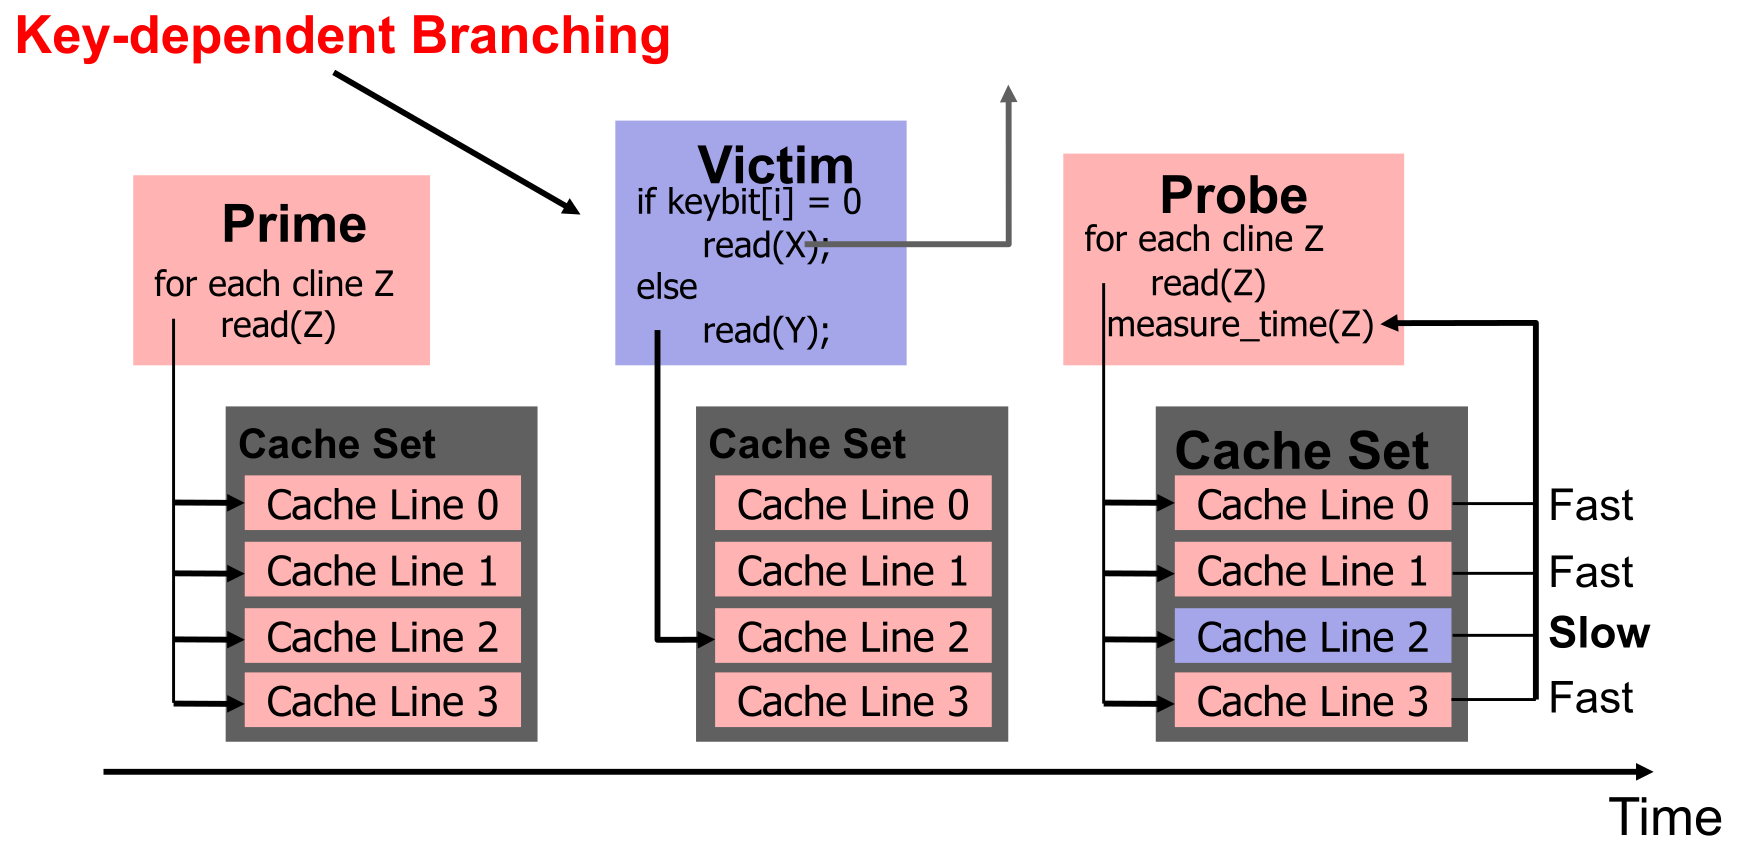
\includegraphics[width=\columnwidth]{sidechannel-prime-probe.png}
\subsubsection{Variants}
\begin{enumerate}
  \item \textbf{Data access} depends on secret data: Data access patterns
    in the cache leak information about the secret
  \item \textbf{Control flow} depends on secret data: Code access
    patterns in the cache leak information about the secret
\end{enumerate}
\subsubsection{Cache Timing Attack on AES}
\textbf{Background}\\
During the execution of AES secret key is used to
index arrays (S-boxes). The time to lookup an array element depends
on whether this element of the S-box has partially or entirely been loaded into the
cache.
\begin{itemize}
	\item Allows complete key recovery.
	\item Problem is in the design, not in the implementation.
\end{itemize}

\textbf{Setting:}
\begin{itemize}
\item Attacker can send messages and observe overall execution time
\item Attacker has same setup (software, hardware) for local tests
Execution
\end{itemize}

\textbf{Attack:}
\begin{itemize}
\item For each byte of the key, one index value will have the slowest lookup.
\item The total execution will be slow
\item Find this index value
\item (try many messages locally)
\end{itemize}


\subsubsection{Protecting}
\begin{itemize}
  \item \textbf{Basic principle:}
    Try to eliminate secret-dependent cache access patterns
  \item Specific defenses exist, but eliminating all secret-dependent
    branching (code and data) is difficult and expensive…
  \item Most CPUs have special AES hardware  $\Rightarrow$ not vulnerable.
\end{itemize}

\subsection{Power Analysis Attacks}
Mainly used on Smartcards, RFID chips, Sensor Nodes
\begin{itemize}
  \item The attacker needs to have physical access
  \item Measures the consumed power during  operation
\end{itemize}
Square-and-multy in RSA is vulnerable through simple power analysis.
\subsubsection{Protection}
Goal: Elimination or significant reduction of the correlation between operand
values and power consumption.
\begin{itemize}
	\item Random change of power consumption in time
	\item Noise generator
	\item Physical shielding
	\item Software balancing
	\item Hardware balancing
\end{itemize}

\subsection{Acoustic Attacks}
\begin{itemize}
	\item High-frequency sounds caused by vibration of
electronic components
\item \textbf{Different keys cause different sounds}
  \item Can extract RSA keys based on sound
\end{itemize}

	% !TeX root = ../summary-syssec.tex

\section{Tamper Resilience}
\subsection{Classification}
\begin{itemize}
  \item Tamper resistant
    \begin{itemize}
      \item Bank vault approach
      \item Purpose: Prevent/slow down of break-in
    \end{itemize}
  \item Tamper responding
    \begin{itemize}
      \item Alarm approach
      \item Erasure or destruction of secret data
      \item Purpose: real-time-detection
    \end{itemize}
  \item Tamper evident
    \begin{itemize}
      \item If a break-in occurs, evidence of the break-in is left behind.
      \item Purpose: detection of intrusion
    \end{itemize}
\end{itemize}

\subsection{Smartcards}
\begin{itemize}
  \item Limited tamper resistance
  \item PIN + card possession enable user authentication
  \item Card holds a key
\end{itemize}
\subsubsection{Memory Read-out Attack}
Attacker initiates the protocol (the same protocol that the legitimate reader would),
and when the CPU accesses memory to get the key, it reads the key from the
memory bus.

\textbf{Protections:}
\begin{itemize}
  \item read critical keys from memory only after authenticating
    that they are talking to ATM.
\end{itemize}

\subsection{Hardware Security Module}
\begin{itemize}
  \item Tamper resistance
  \item Limited set of functions
  \item No support for exporting the key
\end{itemize}

\subsection{Glitch Attacks}
In a glitch attack, attacker deliberately generate a malfunction that
causes one or more flipflops to adopt the wrong state.\\
$\Rightarrow$ Replace a single critical machine instruction with arbitrary one.

\textbf{Example:}
\begin{lstlisting}
a = answer_address
b = answer_length
if (b == 0) goto 8
transmit(*a)
a = a + 1
>-> b = b - 1 <-< % prevented by glitch
goto 3
...
\end{lstlisting}
Clock-signal glitches are currently the most used. They temporarily increase
the clock frequency, such that some flipflops sample their input before the new
state has reached them.

\subsubsection{Protection}
\begin{itemize}
  \item  Low and high voltage sensors
  \item Frequency sensors and filters
  \item Light sensor
  \item Glitch sensor
  \item Software countermeasures
\end{itemize}

\subsection{API Attacks}
\subsubsection{Background}
A security API is the software layer through which the module's functions are
exposed to the external world.
\begin{itemize}
  \item The HSM is secure
    \begin{itemize}
      \item Protects Contents (Keys, Secrets, PINs)
      \item Can’t break in (Tamper-Evident)
    \end{itemize}
  \item Trick the HSM into leaking the secrets by
    sending the right requests!
  \item Most taper resistant devices are vulnerable to API attacks
\end{itemize}

\subsubsection{PIN Verification at a Bank}
\textbf{Inputs:}

\begin{itemize}
  \item Encrypted PIN, Account Number (PAN)
  \item Decimalization Table, PIN Offset
\end{itemize}
\textbf{Attack Idea:} Supply different decimalization table and PIN offset
\begin{center}
  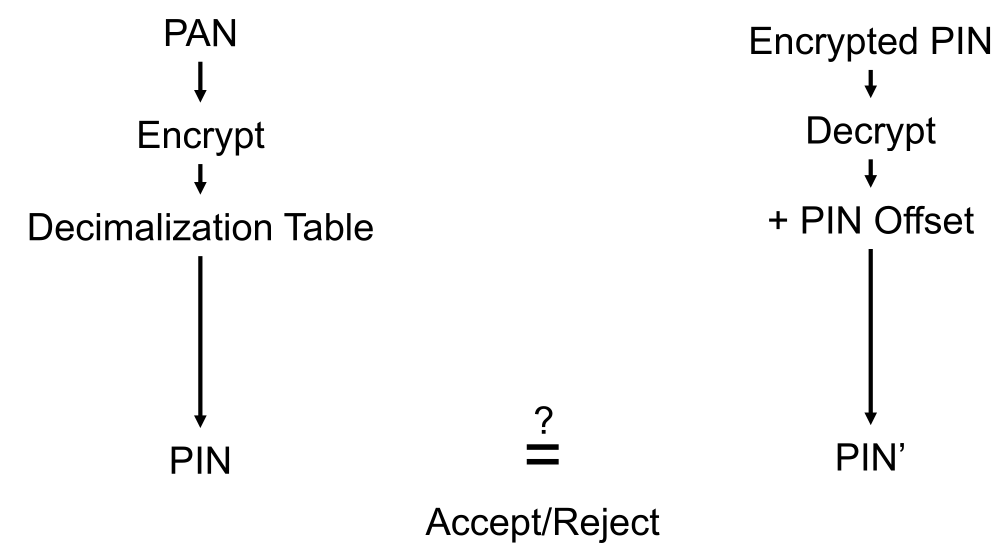
\includegraphics[width=0.6\columnwidth]{tamper_resilience_PIN-attack.png}
\end{center}

\subsubsection{Chip and PIN}
Man in the middle attack:
\begin{center}
  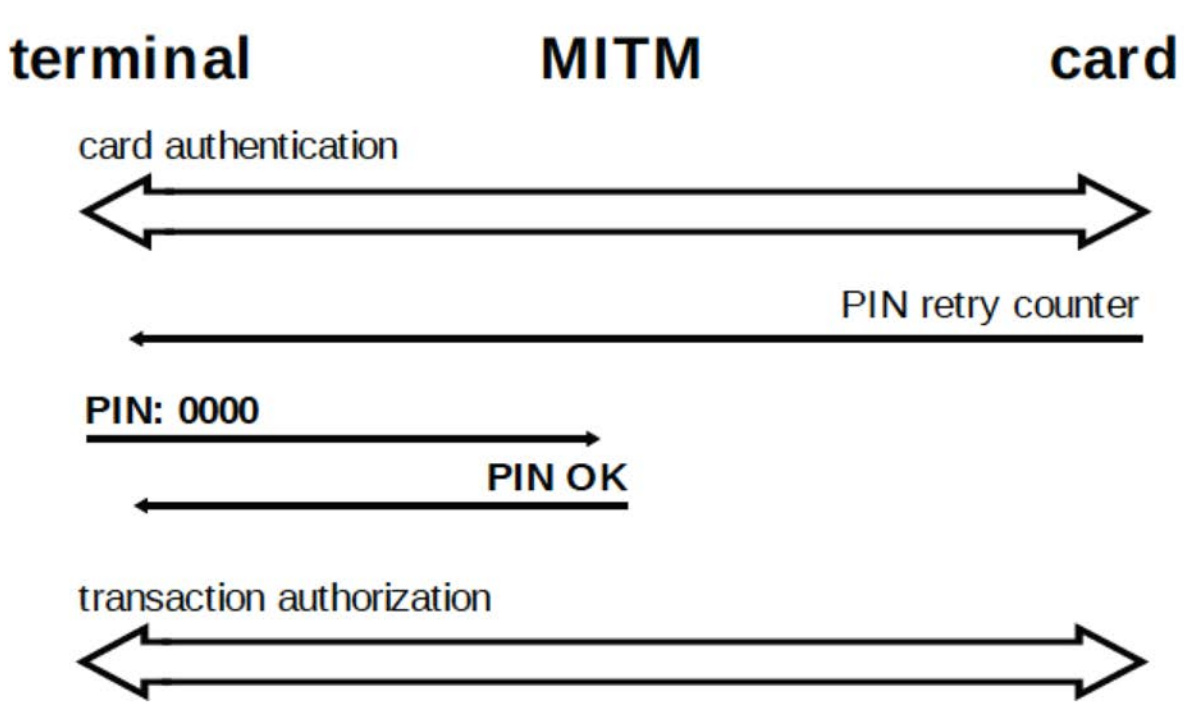
\includegraphics[width=0.5\columnwidth]{tamper_resilience_chip-and-pin.png}
\end{center}
Before the transaction, the MITM tells card that transaction will be signed on
paper $\Rightarrow$ No PIN required.

\subsection{Protection}
\begin{itemize}
  \item Access Control
  \item Limit functionality
    \begin{itemize}
      \item E.g. Do not allow other decimalization tables
    \end{itemize}

\end{itemize}

	% !TeX root = ../summary-syssec.tex

\section{Security on Commodity Systems}
\subsection{Application Security}
\subsubsection{Properties}
\begin{description}
  \item[Launch-time integrity:] \textit{correct} application was started
  \item[Run-time isolation:] no interference from malicious software or
    peripherals
  \item[Secure persistent storage] Confidentiality, integrity protection of
    data
\end{description}


\subsection{OS-based Security}
\subsubsection{Privilege Rings}
\begin{center}
  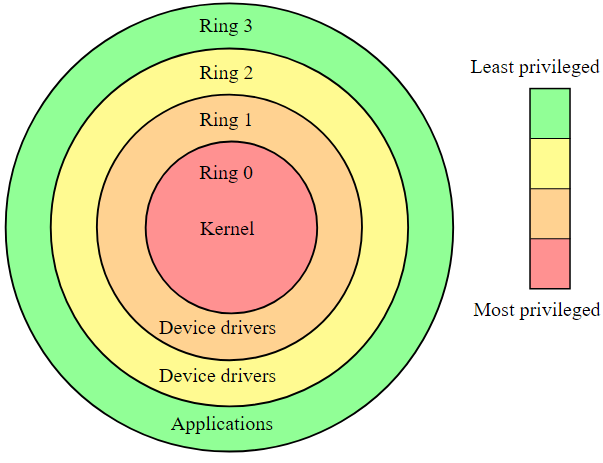
\includegraphics[width = 0.6\columnwidth]{commodity_systems_privilege-rings.png}
\end{center}
\begin{itemize}
  \item Today, only rings 0 and 3 are used; 1 - 2 part of kernel
  \item Main use: limiting access to privileged instructions, I/O-ports
\end{itemize}


\subsubsection{Paging-based Security}
Security-relevant data in page table entries:
\begin{description}
  \item[Supervisor bit:] if set, this page is accessible only in ring 0
    (isolates OS from applications)
  \item[RW bits:] to distinguish between read-only and writeable pages
  \item[Execution disable (ED) bit:] if set, the page is not executable
    (prevents run-time code injection)
\end{description}


\subsubsection{Firewire (DMA) Attack}
\begin{description}
  \item[Background:] Firewire  allows for fast communication speeds
    between devices, uses DMA (Direct Memory Access)
  \item[Idea:] Access to RAM is controlled by CPU. This can be circumvented by
    DMA.
  \item[Attack:]\hfill
    \begin{itemize}
      \item The attacker uses a Firewire cable to connect to a (locked) PC
	and issue a DMA request to fetch the contents of RAM
      \item Later on it can look in the collected data and find out keys and
	other passwords
    \end{itemize}
  \item[Protection:] \hfill
    \begin{itemize}
      \item Have no Firewire ports, but there are other ports for
	similar attacks.
      \item OS sets up a IOMMU (Input–output memory management unit) to control
	DMA access to physical memory.
    \end{itemize}
\end{description}


\subsubsection{Disk Encryption}
\begin{description}
  \item[Idea:] Disk is encrypted and unlocked by a secret key.
    \begin{itemize}
      \item Data on disk is allways encrypted.
      \item File system is completely unaware:
	\begin{center}
	  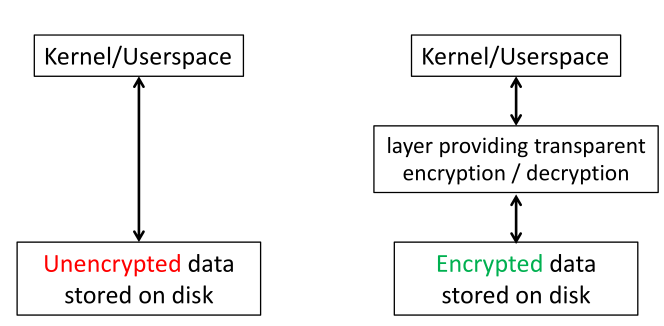
\includegraphics[width=0.6\columnwidth]{commodity_systems_disk-encryption.png}
	\end{center}
    \end{itemize}

  \item[Simple Approach:] Use password only $\Rightarrow$ can be
    bruteforced
  \item[Better Approach:] Store disk encryption key in a secure element
    (TPM) $\Rightarrow$ requires more hardware support.
\end{description}


\subsubsection{Cold Boot Attack on Disk Encryption}
\begin{description}
  \item[Idea:] \hfill
    \begin{itemize}
      \item encryption key is kept in memory
      \item DRAM keeps it's state for a while without refresh, and
	longer if it is cold.
    \end{itemize}
  \item[Attack:] \hfill
    \begin{itemize}
      \item Remove power
      \item Cool down RAM
      \item Plug RAM to another platform / Boot with a USB and attack
	tools to copy memory content
      \item Recover key (part in memory with high entropy)
    \end{itemize}
  \item[Protection:] \hfill
    \begin{itemize}
      \item Erase key from memory on every suspend
	\begin{itemize}
	  \item does not help sudden power loss
	\end{itemize}
      \item Physical protection
      \item Avoid to have key in memory
    \end{itemize}
\end{description}


\subsubsection{Chain of Trust}
\begin{center}
  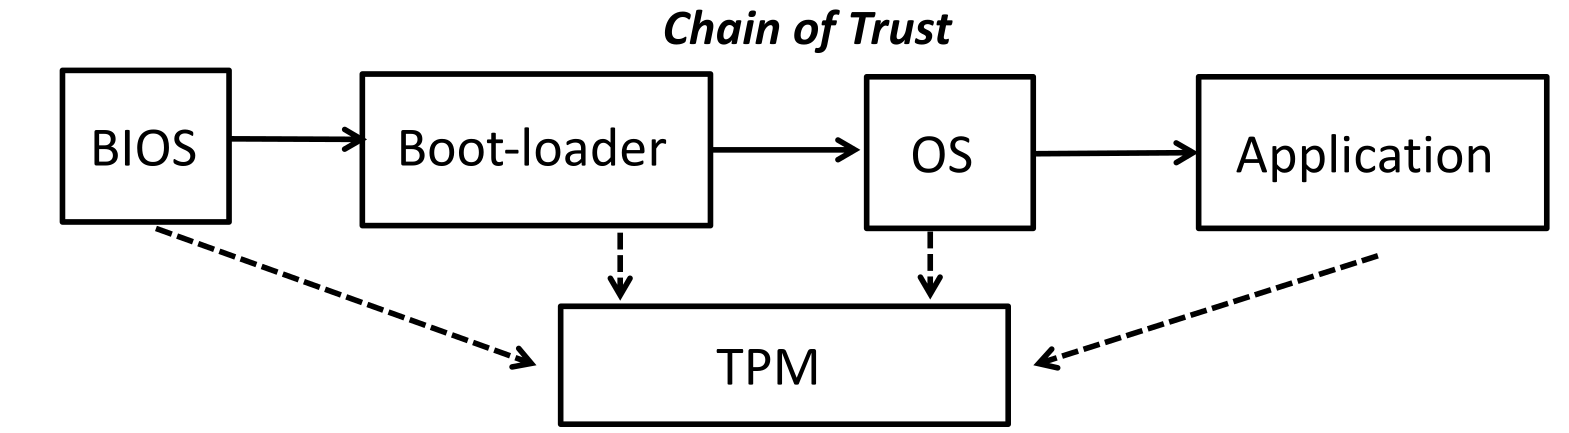
\includegraphics[width=0.7\columnwidth]{commodity_systems_chain-of-trust.png}
\end{center}
\begin{description}
  \item[Secure Boot:] OS boots only if the chain of trust is valid
  \item[Authenticated boot:] System records chain of trust but OS boots
    even if the chain is invalid
\end{description}


\subsection{Storage protection on smartphones}
\subsubsection{Background}
\begin{itemize}
  \item Encrypt with user-provided PIN
  \item no TPM available
  \item Approach:
    \begin{enumerate}
      \item At boot the OS asks PIN code from user
      \item PIN is given to the CPU
      \item CPU derives storage encryption key from PIN and processor key
    \end{enumerate}
    $\Rightarrow$ Prevents brute-forcing of extracted storage
  \item storage must be decrypted on the same device where the CPU is
  \item A counter indicates how many attempts are left.
\end{itemize}

\subsubsection{NAND Mirroring Attack}
\begin{enumerate}
  \item  Eavesdropping:\\
    Find the communication protocols and the communication speeds
  \item Backing Up:\\
    Create a copy of the NAND chip
  \item Restoring:
    \begin{itemize}
      \item Power on phone
      \item Enter 6 PINs
      \item Power down
      \item Take out NAND and restore modified parts from backup
      \item Put NAND back into phone
      \item Repeat
    \end{itemize}
  \item OR Cloning:
    \begin{itemize}
      \item Arbitrarily many clones can be created
      \item Always plug in a new cloned chip
    \end{itemize}
\end{enumerate}

	% !TeX root = ../summary-syssec.tex

\section{Intel SGX (Software Guard Extension)}
\subsection{Basics}
\begin{itemize}
  \item Security enhancements in Intel CPUs
  \item Enclave = security-critical part of the application
  \item Main goal:
    \begin{itemize}
      \item Enable secure execution in otherwise untrusted platforms (OS, ...)
      \item Enclave data confidentiality and execution integrity
    \end{itemize}
  \item Idea: Reduce TCB and trust boundary.
    \begin{center}
      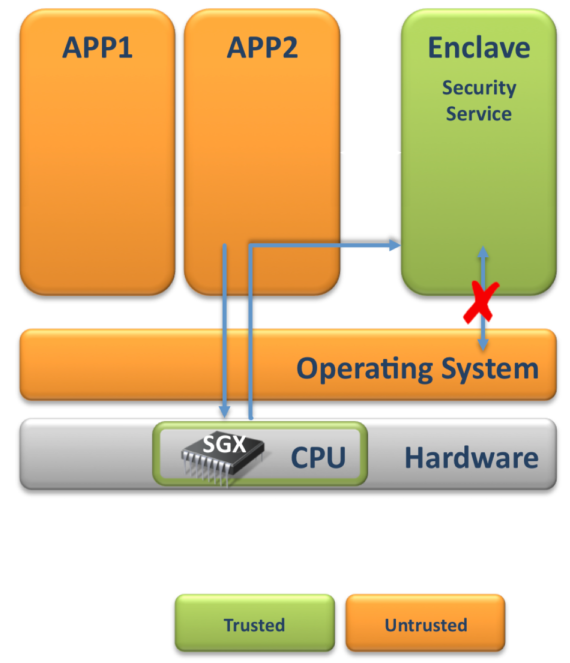
\includegraphics[width=0.3\columnwidth]{sgx_idea.png}
    \end{center}
  \item Unique set of keys are burned into the processor.
  \item Parallel Execution of different Enclaves possible.
\end{itemize}

\subsection{Enclave Creation}
\begin{center}
  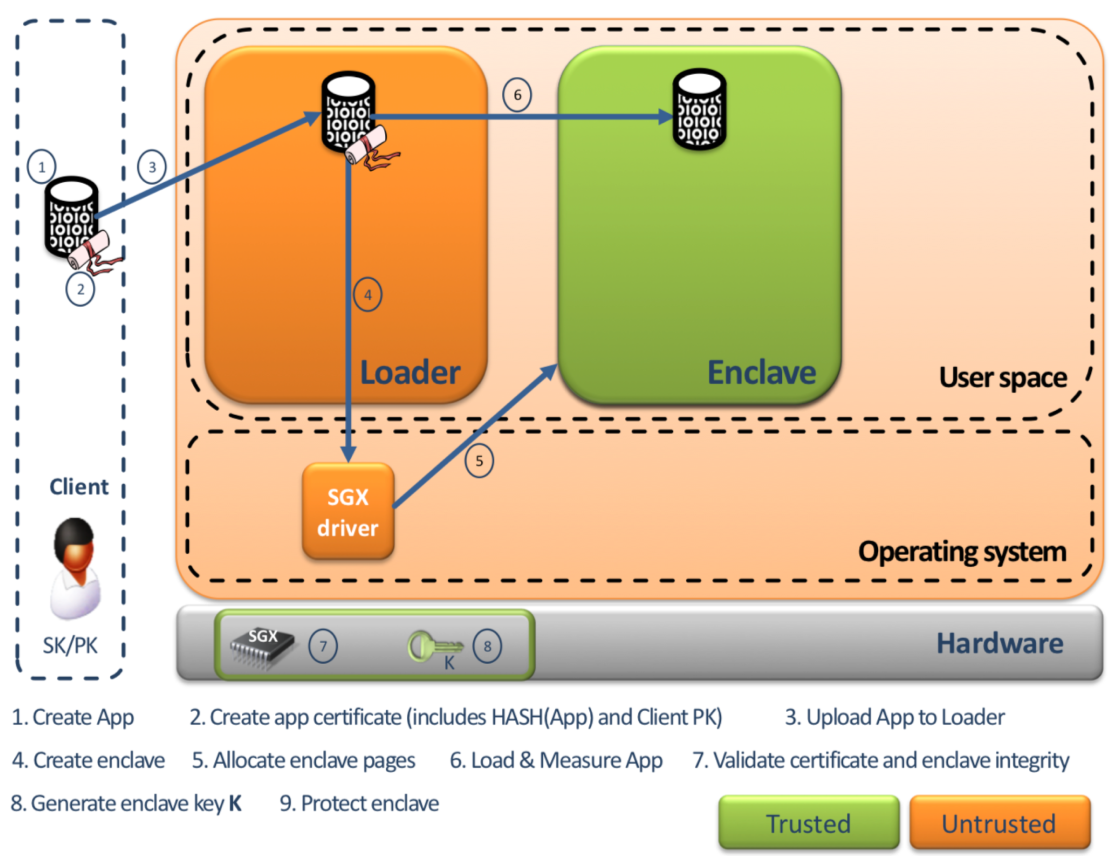
\includegraphics[width=0.9\columnwidth]{sgx_create_enclave.png}
\end{center}

\subsection{Sealing}
\begin{itemize}
  \item Store encrypted confidential data on disk. Only Enclave can access it.
  \item Enclave has no direct access to IO / storage.
  \item Same Enclave ID on the same platform can unseal it's sealed data.
  \item Enclave will loose state across reboots, but can unseal it's sealed
    state.
\end{itemize}


\subsection{Attestation and secure communication}
\begin{itemize}
  \item Two enclaves can communicate to securely over an untrusted channel.
  \item Remote Attestation allows Enclave to check whether other instance is a
    valid and secure SGX Enclave.
\end{itemize}

\subsection{Application: DelegaTEE}
\begin{itemize}
  \item Owner's credentials remain confidential.
  \item The Owner can restrict access to his account (in time, actions,
    ...)
  \item Difficult to distinguish between access by the
    Delegatee and Owner
  \item Functioning:
    \begin{center}
      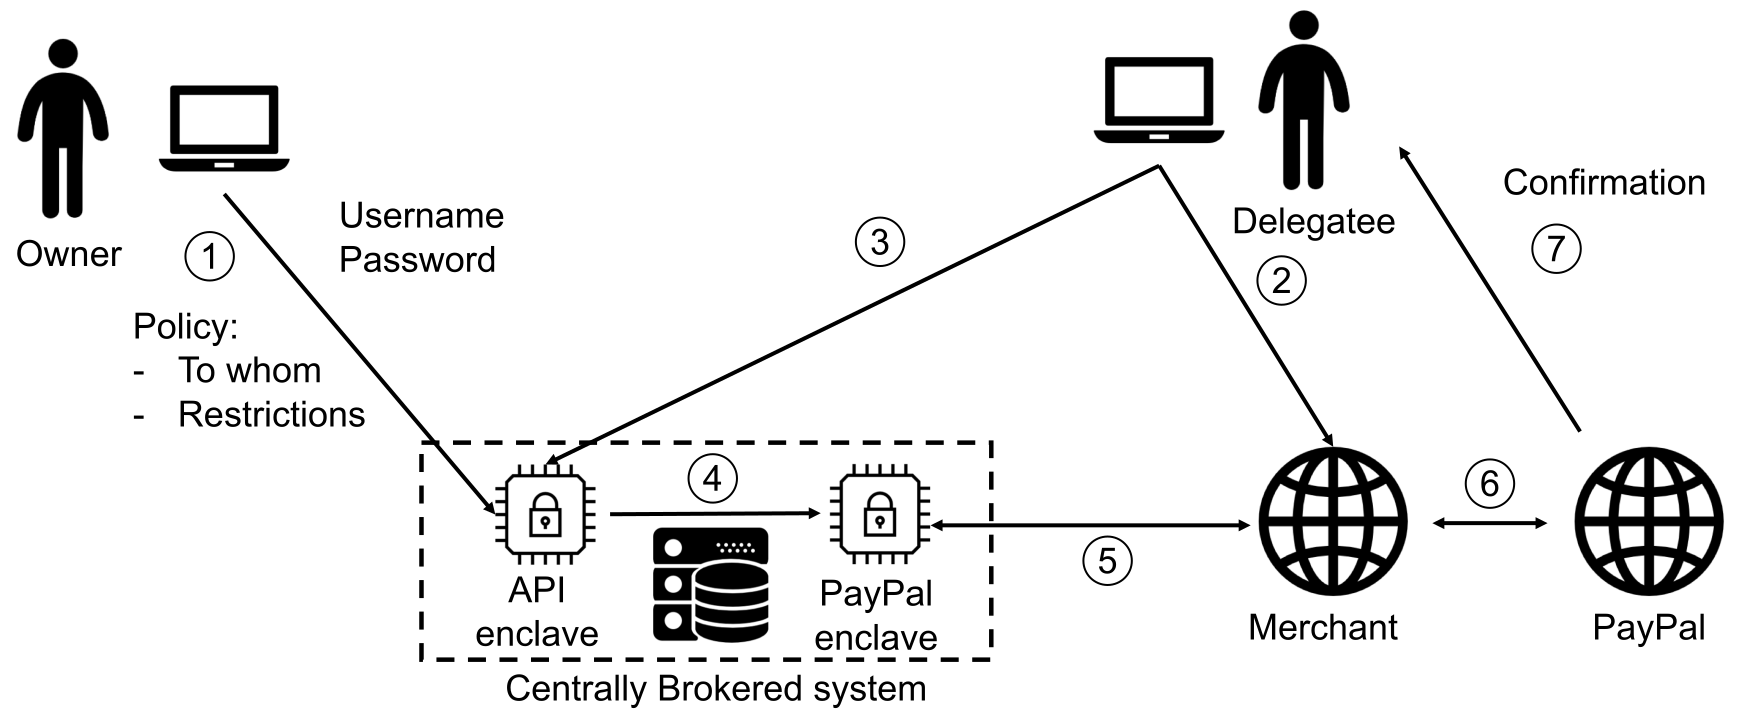
\includegraphics[width=0.9\columnwidth]{sgx_delegatee.png}
    \end{center}
  \item Applications: Email access, website access, e-banking, paypal
  \item May undermine service (e.g. Netflix) and create market for sharing
    economy
  \item Two systems possible: centrally brokered or decentralized
    peer-to-peer
\end{itemize}

\subsection{Attacks}
\subsubsection{Cache-timing attack}
\begin{itemize}
  \item  PMC
    \begin{itemize}
      \item Use Performance Monitoring Counters (PMC) to count cache misses
	(instead of timing L1 vs. L2)
      \item Enabled by privileged adversary
    \end{itemize}
  \item  isolate victim
    \begin{itemize}
      \item Assign the attack process and victim enclave to separate core
      \item Reduces noise
    \end{itemize}
  \item  hyper-threading
    \begin{itemize}
      \item Run uninterrupted victim enclave and attacker in parallel
      \item Complicates attack detection
    \end{itemize}
  \item Attack target
    \begin{itemize}
      \item Attack non-cryptographic computations
    \end{itemize}
\end{itemize}
Generic and efficient defenses  are an open problem.

	\section{Meltdown-Spectre Attacks}
\subsection{Meltdown}
\subsubsection{Basics}
Architectural state $\not = $ Microarchitectural state

Cache location depends on actual data address.

\begin{description}
    \item[Page tables] translate virt. address to physical address
    \item[Page table entry (PTE)] includes permission bits and who is allowed to access
    \item[Pipelining] split instruction into
        \begin{itemize}
            \item instr. fetch (IF)
            \item instr. decode (ID)
            \item execute (EX)
            \item memory access (MEM)
            \item write back (WB)
        \end{itemize}
    \item[Out-of-Order execution] parallelize execute stage (EX). Run all instr. without inter dependencies in parallel. Retire in-order.
\end{description}


\subsubsection{Attack}
Idea: Microarchitectural state (caches) is modified even if memory access was not allowed.

\begin{center}
    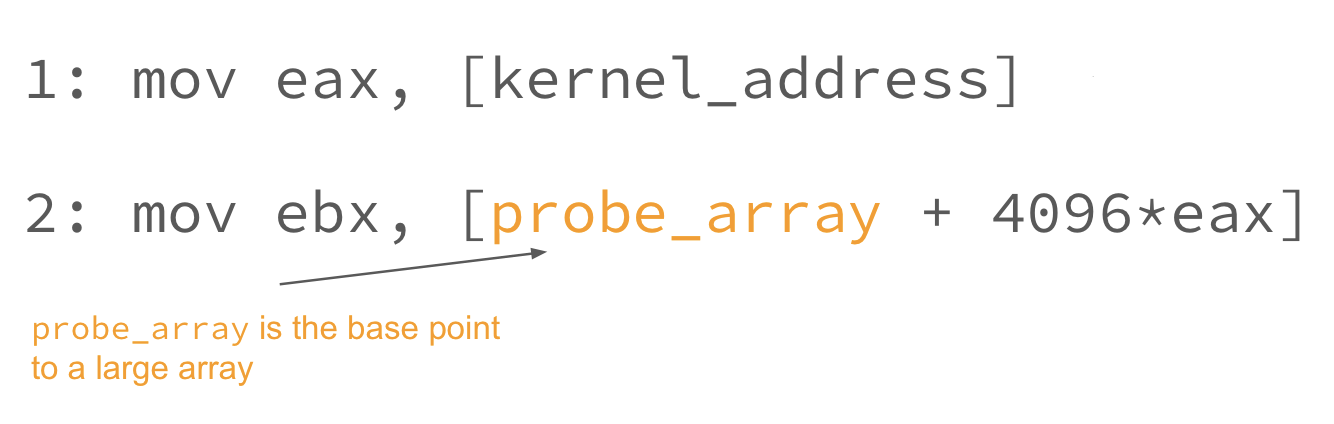
\includegraphics[width=0.8\linewidth]{images/meltdown-cache.png}
\end{center}

\texttt{probe\char`_array} will be accessed at an index which depends on the
secret (e.g. data in kernel address space $[$\texttt{kernel\char`_address}$]$).
Check cache load times for all indices of array to get the index which was accessed by prohibited memory read.

\subsection{Spectre}
\begin{itemize}
    \item based on branch prediction and speculative execution
    \item dynamic predictors use runtime information
    \item Branch Target Buffer (BTB) does not store information about process id or virt. address it belongs to $\xrightarrow{}$ same for each core $\xrightarrow{}$ can be trained by process A but used for B
\end{itemize}

\subsubsection{Spectre 1}
Attacker has control over input used in branch (here \texttt{x}).

\textbf{Can only read memory accessible for process,} but not to the attacker (no privileged read).

\begin{center}
    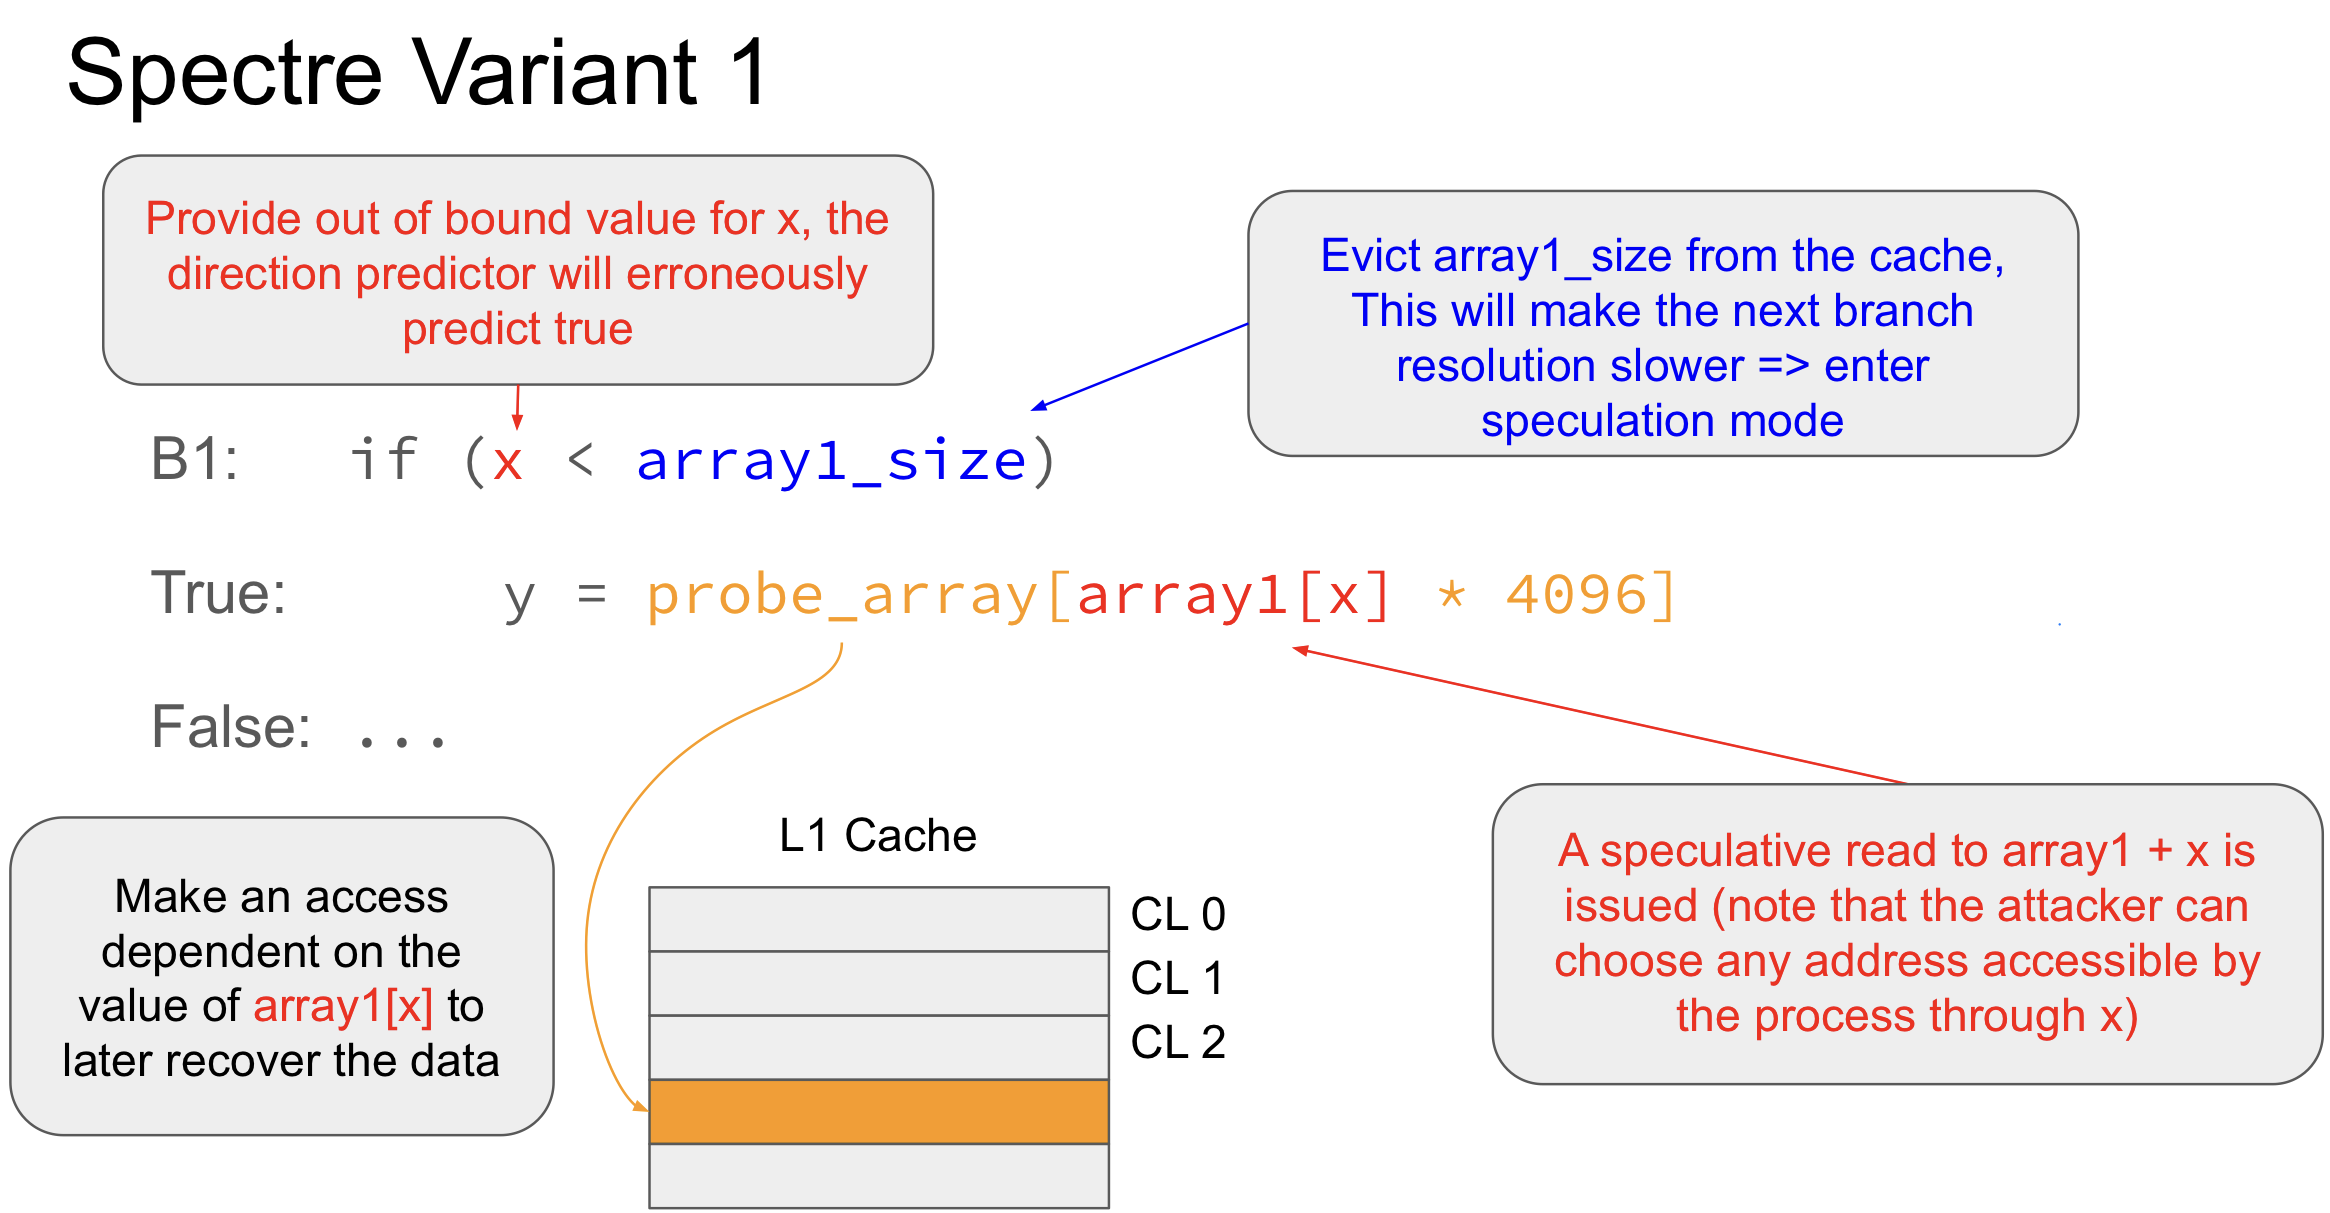
\includegraphics[width=\linewidth]{images/spectre1-overview.png}
\end{center}

\subsubsection{Spectre 2}
Idea: Mistrain BTB to exec. code which creates a side-channel $\xrightarrow{}$
spectre gadget.\\
Unlike Meltdown this does not exploit race condition.

Gadget should:\vspace{-1.5mm}
\begin{enumerate}
    \item exec memory access controlled by attacker's input
    \item exec instr which creates change in microarchitectural state
\end{enumerate}

Attacker needs:\vspace{-1.5mm}
\begin{itemize}
    \item 1 input to select memory location to read
    \item 1 input to control how to leak (e.g. base pointer of \texttt{probe\char`_array})
\end{itemize}

	\section{OS Security}

\begin{description}
    \item[OS Security Goals] secrecy, integrity, availability
    \item[Trust Model] set of SW and data which the system depends on for correct enforcement of security goals
    \item[Threat Model] set of operations available to compromise system
\end{description}

\subsection{Access control}
Whether to allow requests from \textbf{subjects} to perform \textbf{operations} on \textbf{objects}.

\begin{description}
    \item[protection system] defines security requirements of OS. Consists of protection state and protection state operations
        \begin{description}
            \item[protection state] operations a subject can perform on obj.
            \item[protection state operations] enable modification of state
        \end{description}
\end{description}

An access matrix defines which operations a subject can perform on an obj. (subject as row, object as column)
Store by column: ACL (\textbf{A}ccess \textbf{C}ontrol \textbf{L}ist) stored with objects.
Store by column: Capability of a subject
\begin{center}
    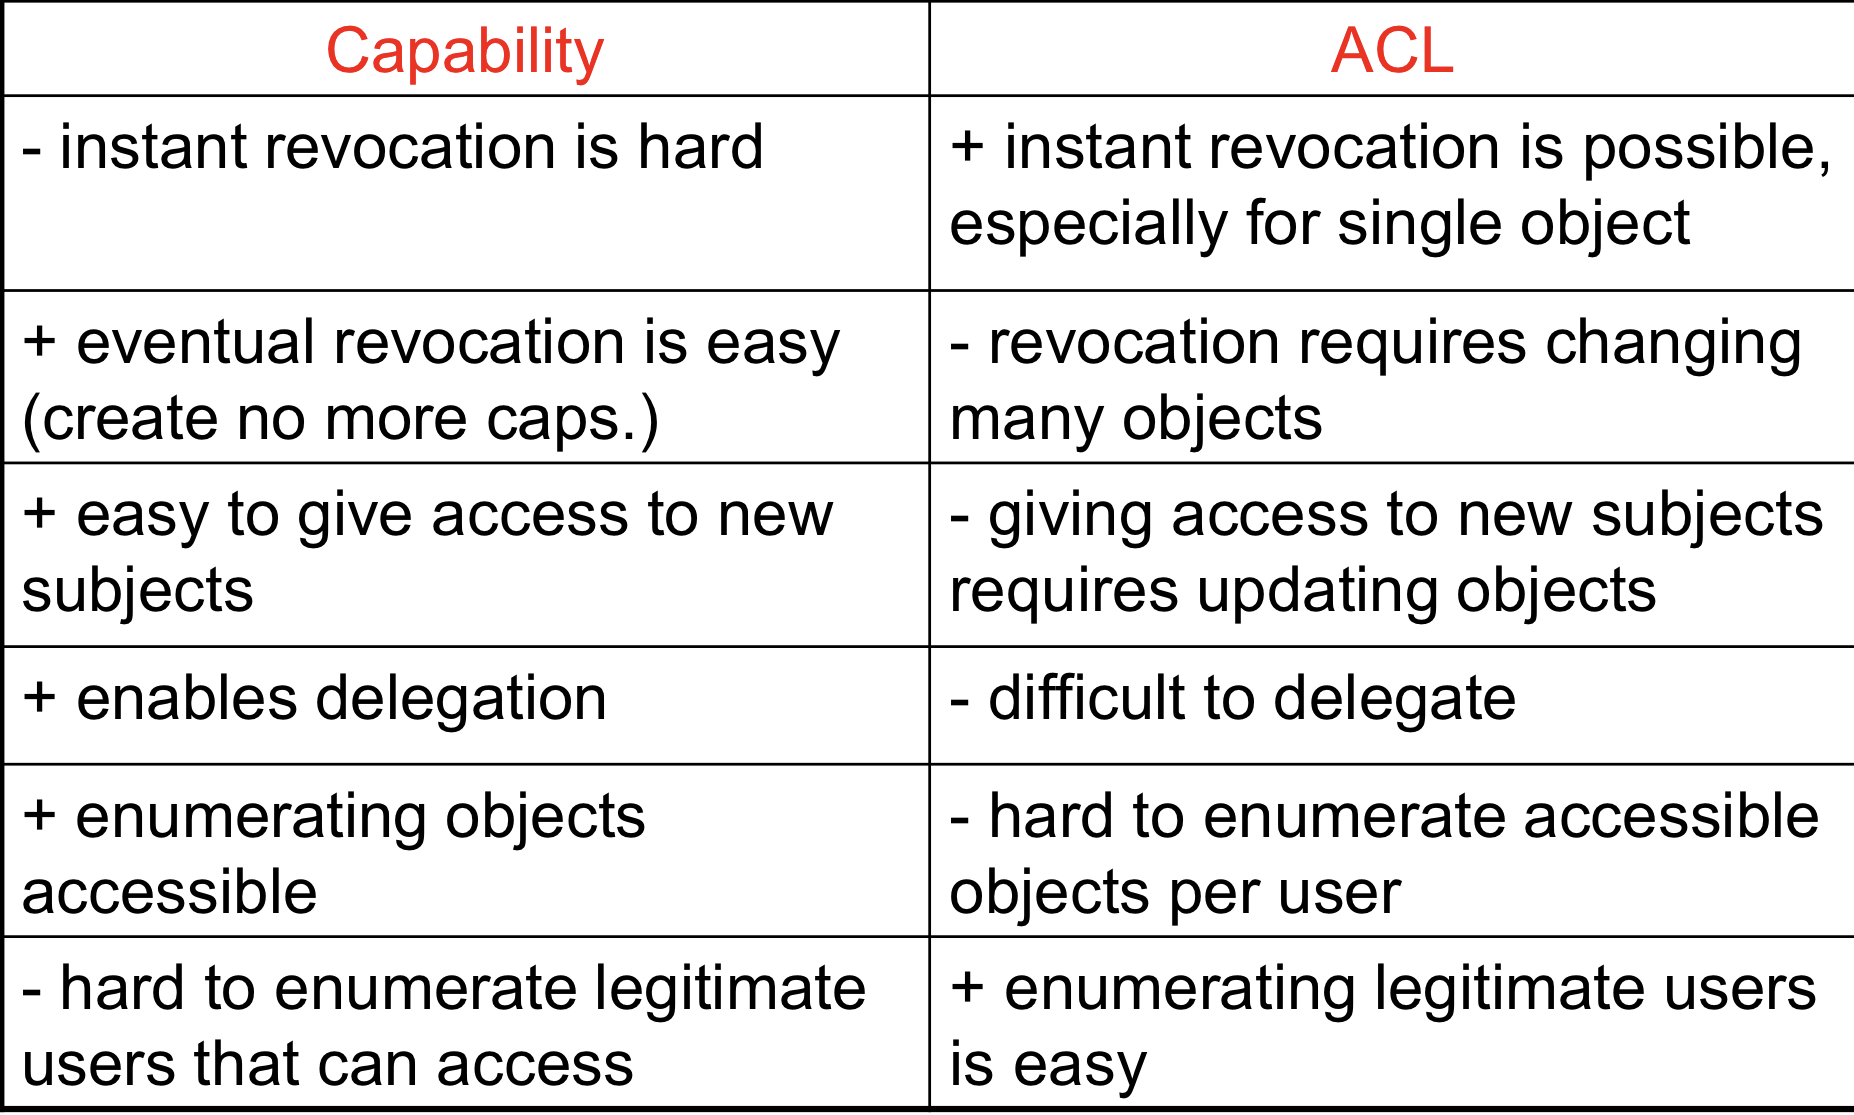
\includegraphics[width=0.65\linewidth]{images/os_sec_capabilities-vs-ACLs.png}
\end{center}

\subsubsection{DAC}
\textbf{D}iscretionary \textbf{A}ccess \textbf{C}ontrol.
Is called discretionary, because subject can pass on his permissions directly/indirectly to other subjects.
\begin{itemize}
    \item allow untrusted processes/users to modify protection state
    \item only works if all processes are harmless and users make no mistakes
\end{itemize}
\subsubsection{MAC}
\textbf{M}andatory \textbf{A}ccess \textbf{Control}

\begin{itemize}
    \item only modifiable by admin
    \item subjects and obj are labels, state represents allowed operations
    \item transition state is legal way to relabel subjects and objs
\end{itemize}

\begin{center}
    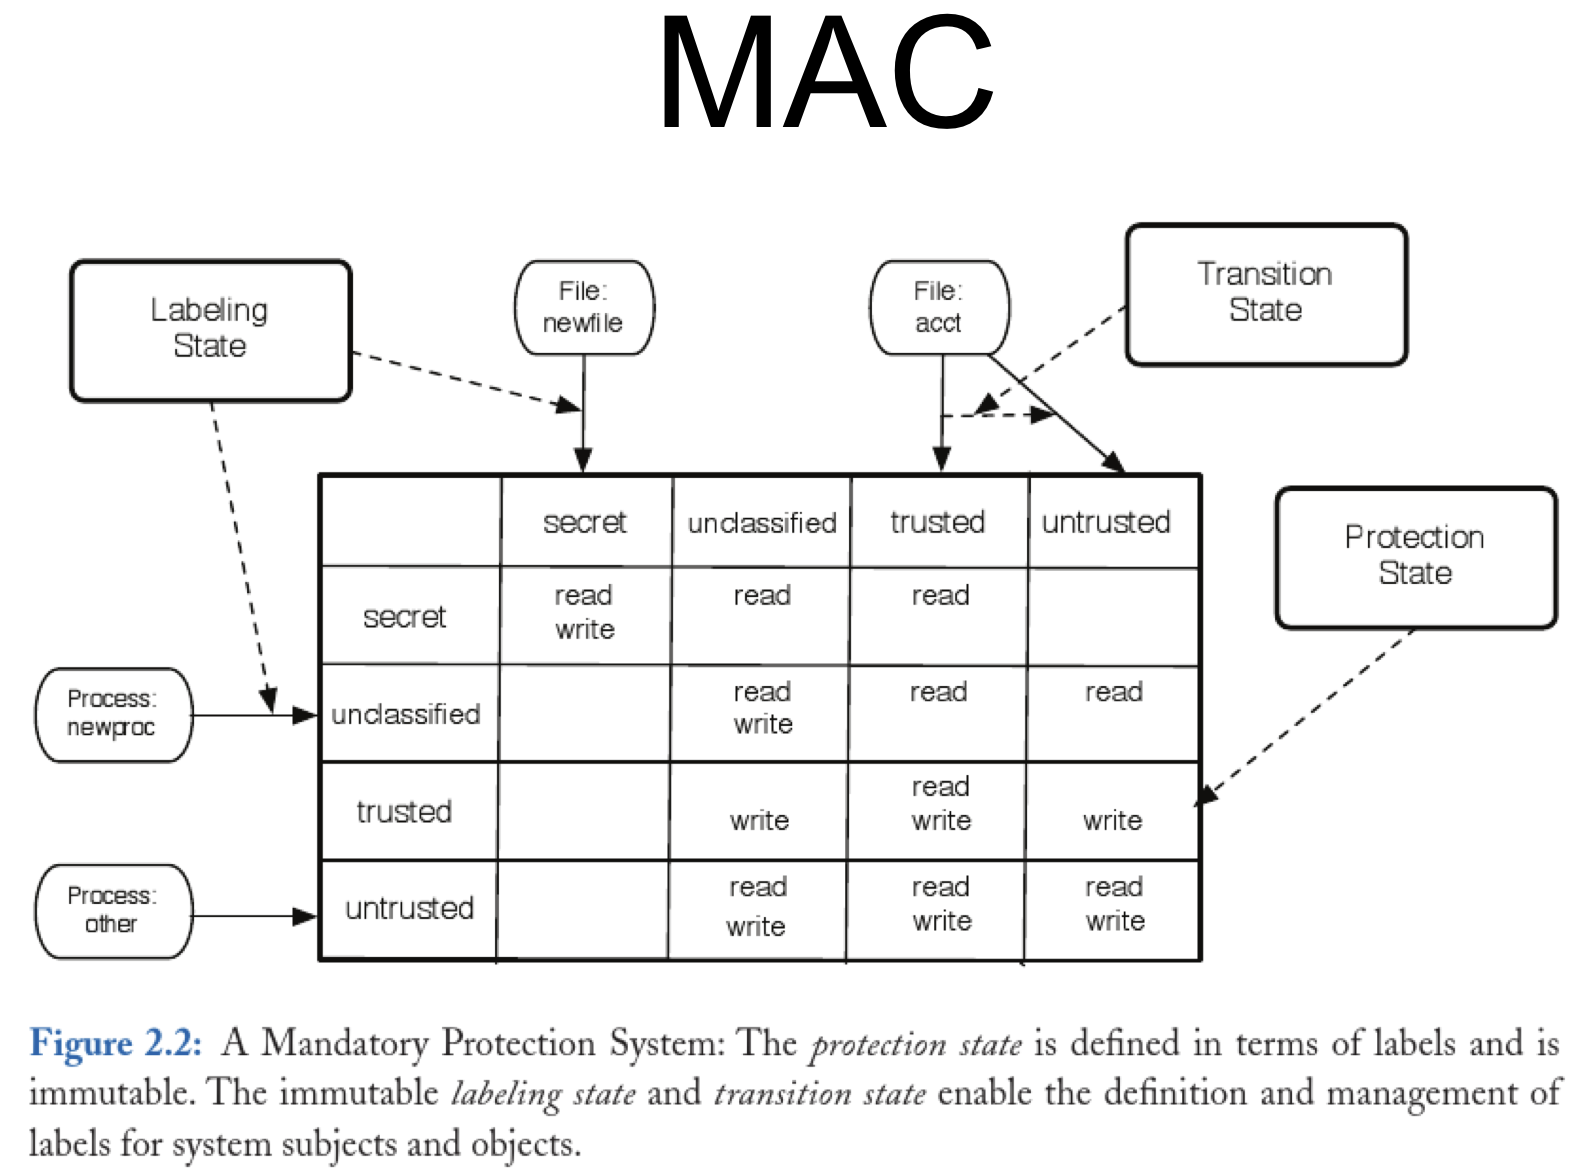
\includegraphics[width=0.9\linewidth]{images/os_sec_MAC.png}
\end{center}

\subsubsection{Reference Monitor}
\begin{description}
    \item[input] request of security sensitive operation
    \item[output] binary answer
    \item[authorization module] converts request into query for policy store
\end{description}

\textbf{Secure OS} iff system uses reference monitor which satisfies:
\begin{enumerate}
    \item complete mediation
    \item tamperproof
    \item verifiable
\end{enumerate}

Does not protect against TOCTTOU attacks.

\subsubsection{Covert Channels}
Capability to transfer information between processes that are not supposed to be allowed to communicate by the security policy.

There are \textbf{storage} and \textbf{timing} channels.

Prevent it by:
\begin{itemize}
    \item memoryless program
    \item isolate program
    \item transitivity (if program A is confined and calls program B, then B must also be confined)
    \item masking (caller determines all inputs to all channels)
    \item enforcement (enforce that input into covert channel conforms with caller's [security] specification)
\end{itemize}

\subsection{Linux Security Model}
Process in user space has access rights based on user ID (UID).

UID 0 is reserved for \texttt{root}.
\begin{description}
    \item[kernel process] can access everything
    \item[root process] can order kernel process to access everything
\end{description}

Kernel verifies permissions before system call! Compares UID and GID (Group ID) of subject and object.

\subsubsection{SELinux}
No default superuser exists, because SELinuxs default is to deny access. Everything must be specifically granted.

\begin{description}
    \item[RBAC] Role based access control
        \begin{itemize}
            \item rules specify roles user can use
            \item rules specify when and where a user can transition into another role
        \end{itemize}
    \item[MLS] multi level security
        \begin{itemize}
            \item handling of classified data where \textit{no read up} or \textit{write down} is allowed
            \item enforce by file system labeling
        \end{itemize}
\end{description}

In SELinux every subject/object has a \textbf{security context} which consists of three labels:\vspace{-1.5mm}
\begin{description}
    \item[user label] on a subject: user privileges, on an object: objects owner
    \item[role label]  on a subject: subject's role, on an object: no meaning (always defaults to \texttt{object\char`_r})
    \item[domain label] set of subjects and objects which are allowed to interact with each other
\end{description}
This is called \textbf{type enforcement}! SELinux can make two types of decisions:\vspace{-1.5mm}
\begin{description}
    \item[access decision] Is subject allowed to do something within it's domain?
    \item[transition decision] Is subject allowed to do somthing in another domain (transition into this domain)?
\end{description}
Hard part is not to grant access to files, but allowing \textbf{safe domain transitions}.

Example rule for passwd (access to shadow file missing):\\
\texttt{allow user\char`_t passwd\char`_exec\char`_t: file $\{$ getattr execute $\}$; \\ allow passwd\char`_t passwd\char`_exec\char`_t: file entrypoint; \\ allow user\char`_t passwd\char`_t: process transition;}

\subsection{Other OSs}
\subsubsection{Qubes}
Security by compartmentalization. 1 qube equals 1 VM.

\subsubsection{Microkernels}
Idea is to minimize TCB. Follows least priviledge principle and removes many parts from kernel space.
\begin{center}
    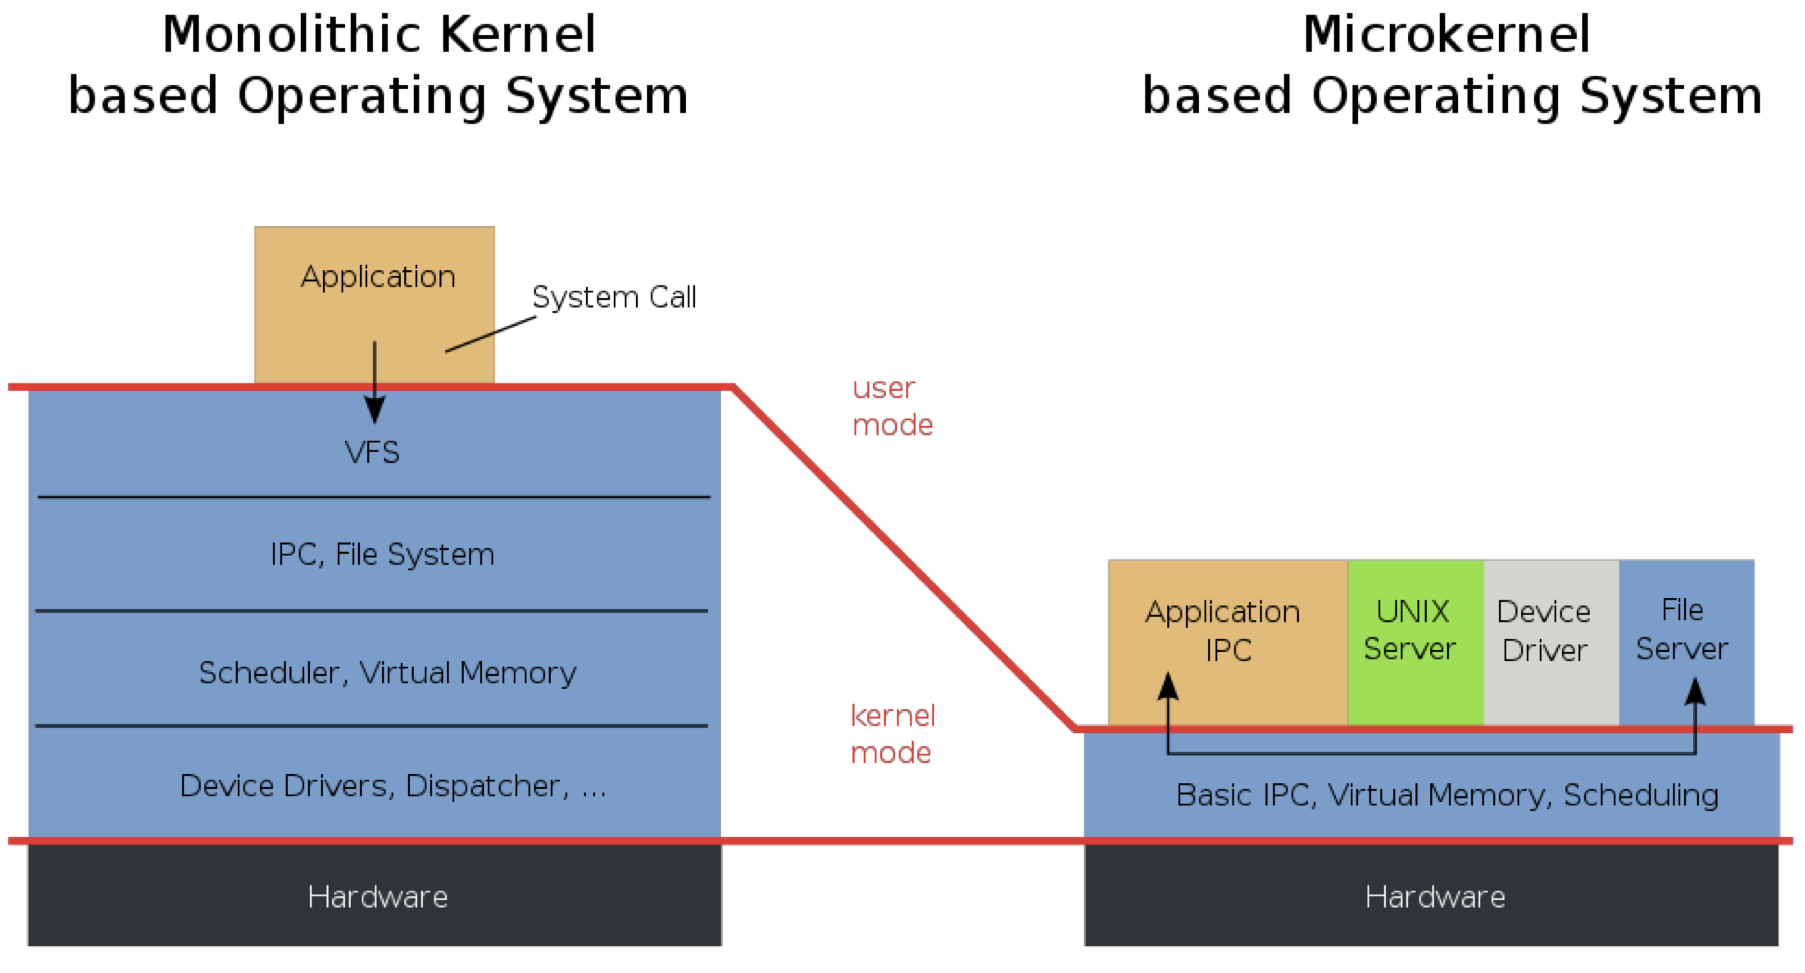
\includegraphics[width=0.8\linewidth]{images/os_sec_MicrokernelVSMonolithic.png}
\end{center}

\textbf{sel4} is a microkernel which focuses on efficency and high assurance. Uses formal verification of code to guarantee correctness w.r.t. specification.
	\section{Mobile Platform Security}
All concepts and issued discussed below are in Android, but may also apply to iOS or other mobile OSs. 
\subsection{Mobile OS Security}
\subsubsection{Basics}
\textbf{Permission-based} access control is key design decision for Android.
Each app has private storage, own process and no communication to other apps (default). If security sensitive operation is required use \textbf{syscall} or \textbf{Android Binders}.

Each app has a designated UID.

\subsubsection{Android Binders}
Allows IPC and RPC (Remote Procedure Call).\\
Example: Accessing location goes through binder which creates channel between unprivileged app and privileged process in application framework.\\
Whether an app can use/call a binder is checked upon invocation based on the requested and granted permissions of an app.
\subsubsection{Permissions}
Three categories of permissions:\vspace{-1.5mm}
\begin{description}
    \item[normal] granted during install by default
    \item[dangerous] prompt user during runtime
    \item[signature] granted during install if signature matches signature of app which declared this permission
    \item[special] must be declared in manifest and granted by user (e.g. system overlays)
\end{description}

Android implements two reference monitors in different places:
\begin{description}
    \item[App-Framework] for system APIs
    \item[Linux-Kernel] for IPC calls to other apps
\end{description}

Problem with permission based design is twofold:
\begin{enumerate}
    \item Users can't associate privacy risks with permissions
    \item Developers tend to request too many permissions
    \item Developers fail to protect IPC interfaces (confused deputy attack)
\end{enumerate}

\subsection{Mobile Hardware Security}
\subsubsection{Trust anchors}
\begin{enumerate}
    \item platform integrity
    \item isolated execution and secure storage
    \item device authentication and remote attestation
\end{enumerate}

\begin{center}
    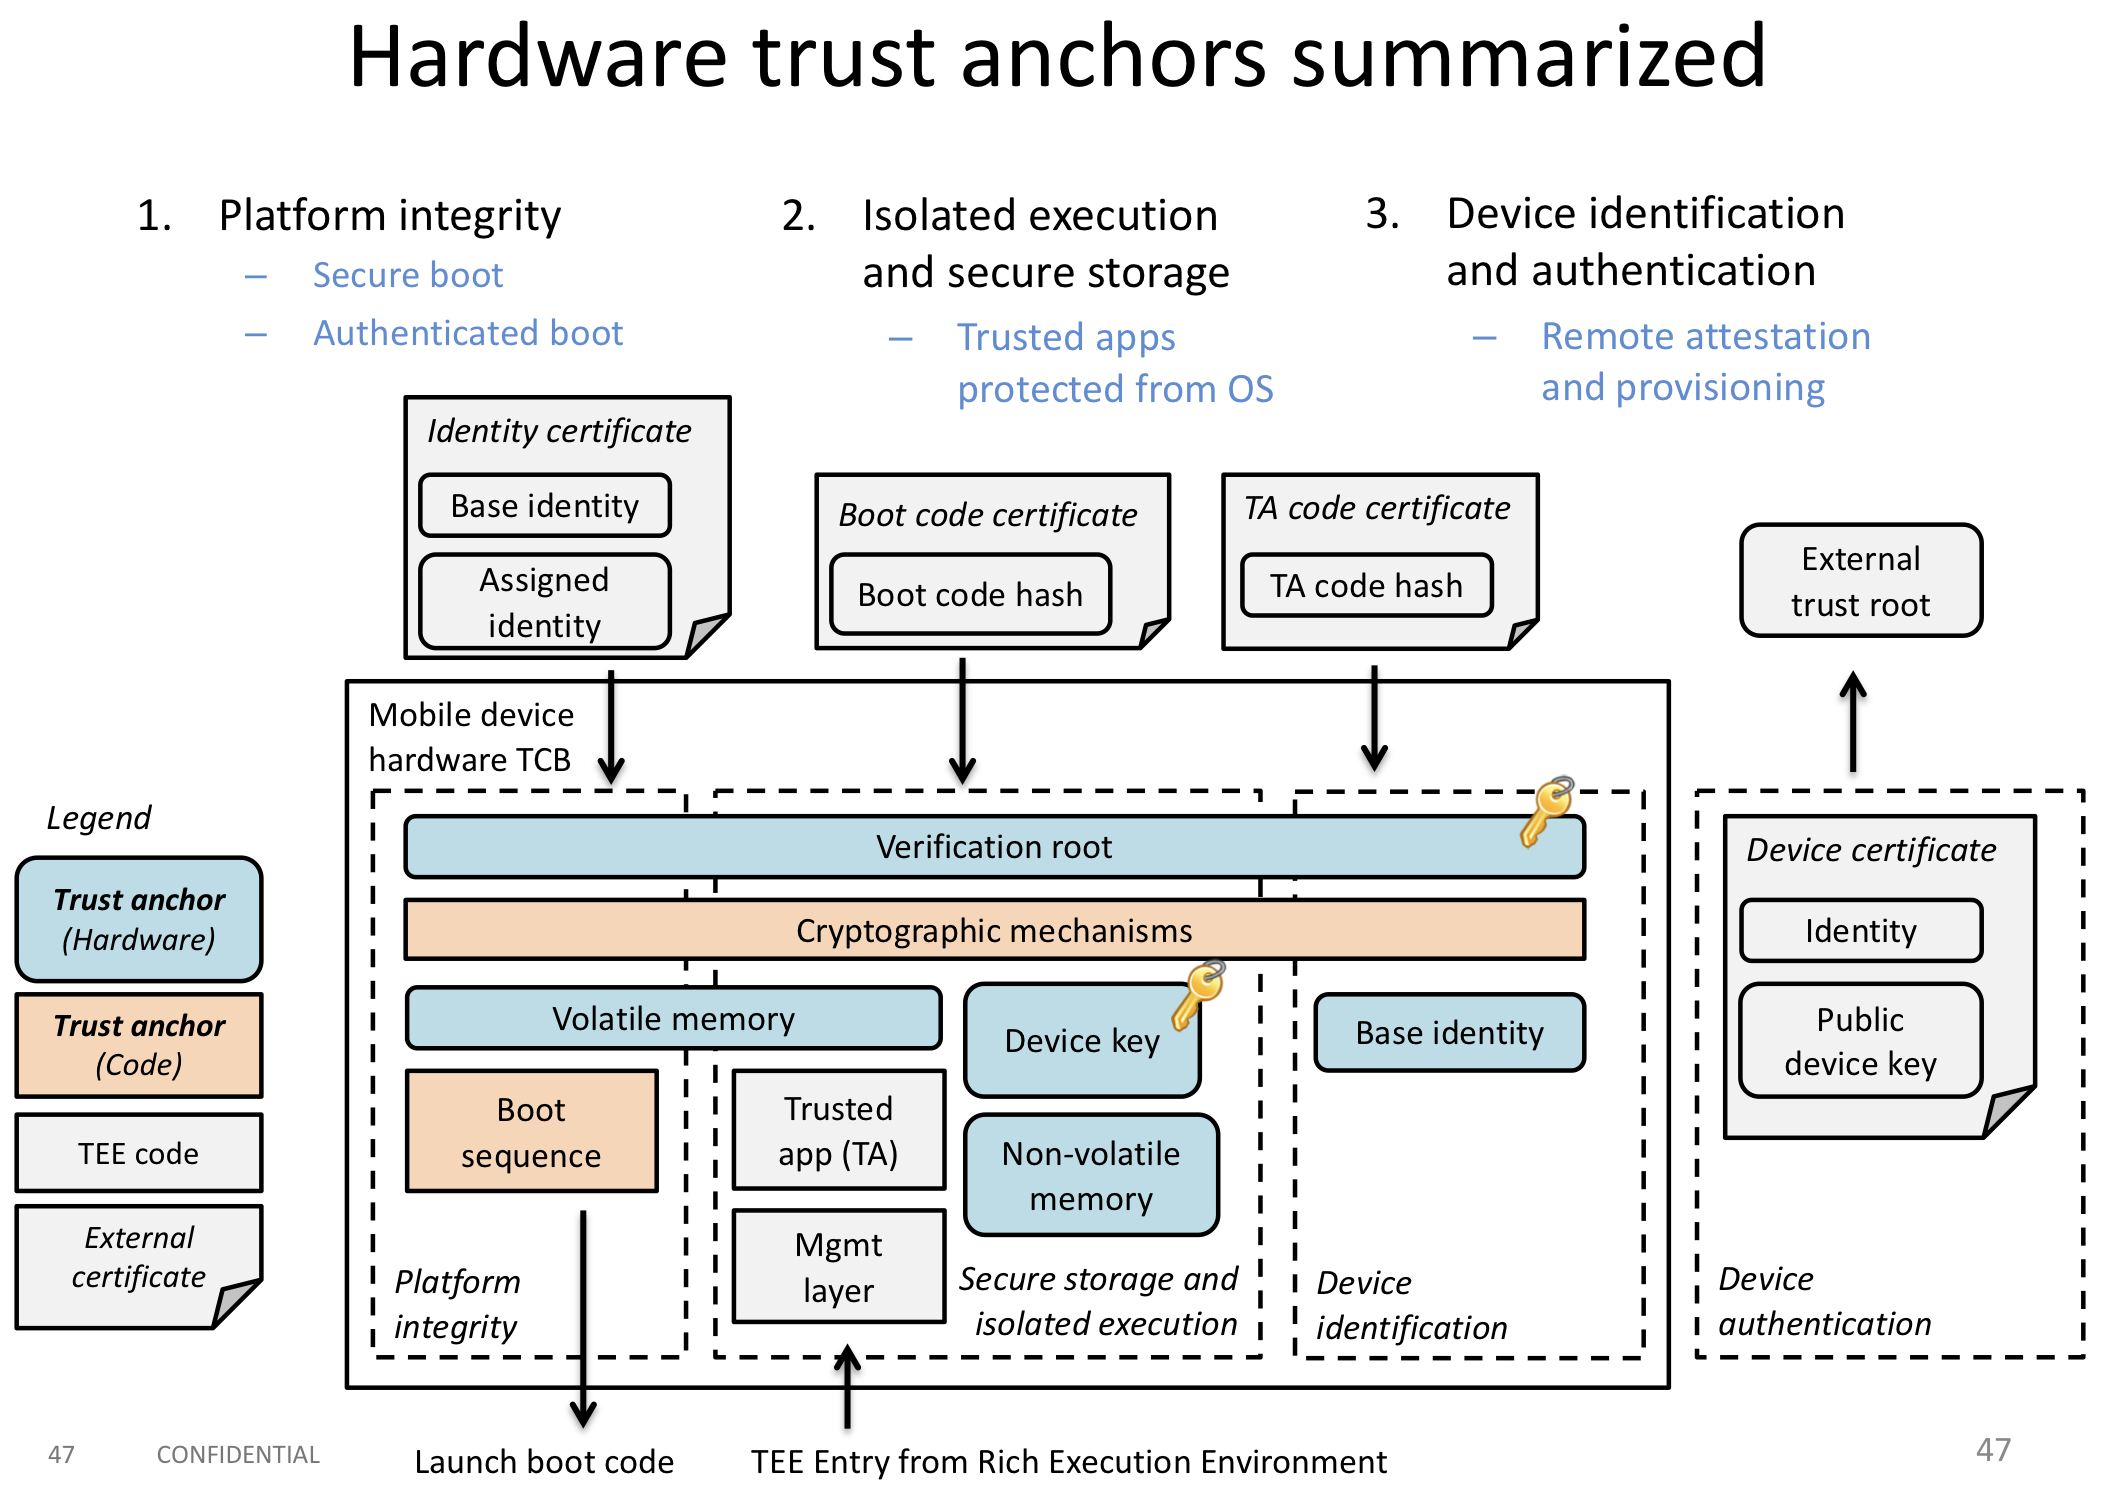
\includegraphics[width=0.85\linewidth]{images/mobile_sec_HardwareTrustAnchors.png}
\end{center}

\subsubsection{TrustZone}
TrustZone apps share the same execution environment. Therefor they mutual trust each other \textbf{or} are isolated by trusted code (TEE management layer).

TrustZone does not specify remote attestation.

App development not open.

TrustZone enables secure communication with external resources (via status flag on bus).

\begin{center}
    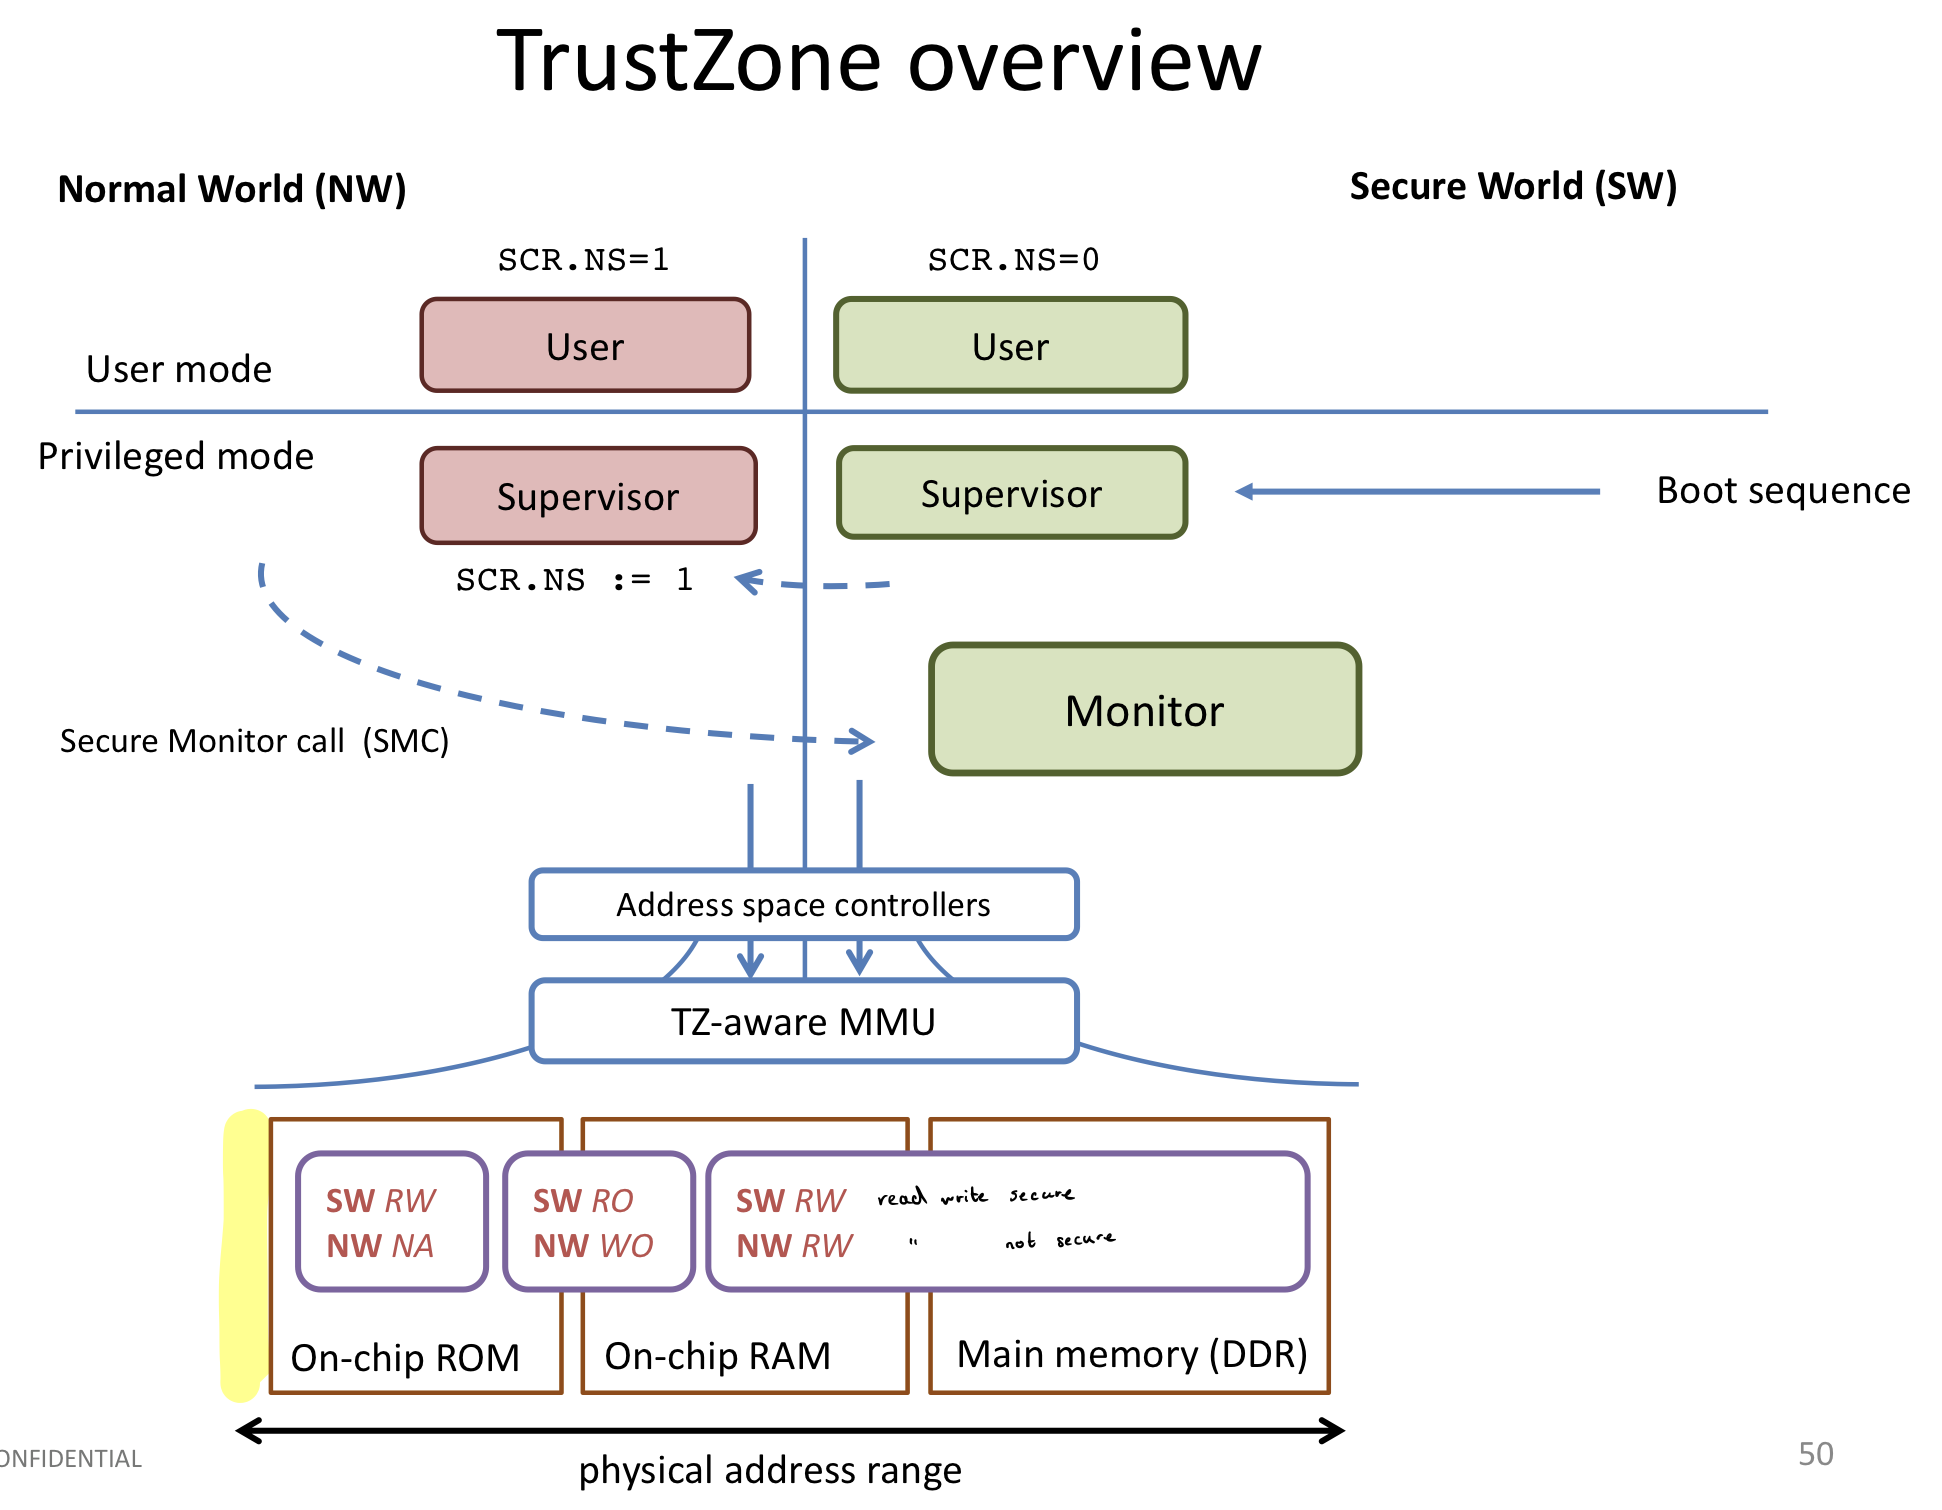
\includegraphics[width=0.8\linewidth]{images/mobile_sec_TrustZoneOverview.png}
\end{center}

Possible attacks against TrustZone: \vspace{-1.5mm}
\begin{itemize}
    \item side-channel similar to meltdown
    \item glitch attacks (e.g. PlunderVolt)
    \item replay attacks (e.g. NAND mirroring)
\end{itemize}
	% !TeX root = ../summary-syssec.tex

\section{Trusted Computing \& Attestation}
Acronyms:
\begin{description}
    \item[TCG] Trusted Computing Group
    \item[TPM] Trusted Platform Module
    \item[PCR] Platform Configuration Register
    \item[TCB] Trusted Computing Base
    \item[SRTM/DRTM] Static / Dynamic Root of Trust for Measurement
    \item[SLV] Secure Loader Block
    \item[TXT] Trusted Execution Technology
    \item[AIK] Attestation Identity Keys (for signing PCRs)
    \item[SRK] Storage Root Key
    \item[IEE] Isolated Execution Environment
    \item[DMA] Direct Memory Access
\end{description}

\subsection{Some Current Approaches}
\subsubsection{Program Code in ROM}
\begin{description}
	\item[Approach:] keep entire program in ROM
	\item[Advantage:] Simple, No injection possible
	\item[Disadvantage:] No updates possible, ROP attacks possible, no
	  isolation
	\item[Verdict:] Not practical
\end{description}

\subsubsection{Secure Boot}
\begin{description}
	\item[Approach:] Only load code with valid signature
	\item[Advantage:] Only approved software loaded
	\item[Disadvantage:] No isolation, difficult to prevent roll-back
	  attacks
	\item[Verdict:] Weak security guarantee
\end{description}

\subsubsection{Virtual-machine-based Isolation}
\begin{description}
	\item[Approach:] Isolate apps by executing in VM
	\item[Advantage:] smaller TCB, isolation between apps
	\item[Disadvantage:] VM still large \& part of TCB, complex
	\item[Verdict:] Step in right direction
\end{description}

\subsection{General Approach}
\begin{enumerate}
	\item Isolated Execution
	\item Remote Attestation
	\item Sealed Storage
\end{enumerate}

\subsection{TPM}
\subsubsection{Basics}
\begin{description}
    \item[Attestation] enables verifier to verify what SW is executing on untrusted device
\end{description}
Adversary model of TPM:
\begin{itemize}
    \item remote attacks
        \begin{itemize}
            \item compromise OS and apps running on the OS
            \item complete control over network communication
        \end{itemize}
    \item local hardware
        \begin{itemize}
            \item generally trusted (because HW attack detection is hard)
            \item attacker can reboot, install malicious SW, attack malicious USB devices
        \end{itemize}
\end{itemize}

Basic TPM functions
\begin{itemize}
    \item PCR registers for integrity measurement chain $PCR_{new} = \texttt{SHA-1}(PCR_{old}|| \texttt{SHA-1}(data))$
    \item on-chip storage for SRK
    \item manufacturer certificate
    \item remote attestation with PCRs and AIK
    \item sealed storage with PCRs and SRK (only accessible under certain integrity measurement)
    \item random number generator
\end{itemize}
TPM is \textbf{passive} component and \textbf{not} tamper proof.

HW attacks possible because TPM is on LPC bus.

\subsubsection{Attested Boot a.k.a. Static Root of Trust}
Measure all executed SW to verify platform configuration. To verify compare measurements to known hashes of trusted SW.

Shortcomings:

\begin{itemize}
    \item TOCTTOU: measurement at load-time and not at runtime (inefficient against dynamic attacks)
    \item coarse-grained: TCP is entire system
    \item no guarantee of execution
    \item every system is different $\Rightarrow$ Database of correct hashes is
      large
\end{itemize}

\subsubsection{Dynamic Root of Trust a.k.a. Late Launch}
Idea: special CPU instruction to create IEE $\xrightarrow{}$ high assurance of code execution and remote attestation

Required computing primitives:
\begin{itemize}
    \item create IEE with \texttt{SKINIT/SENTER}
        \begin{enumerate}
            \item CPU softreset
            \item reset dynamic PCRs
            \item enable DMA protection
            \item send SLB to TPM
            \item execute SLB
        \end{enumerate}
    \item remote attestation
      \begin{center}
	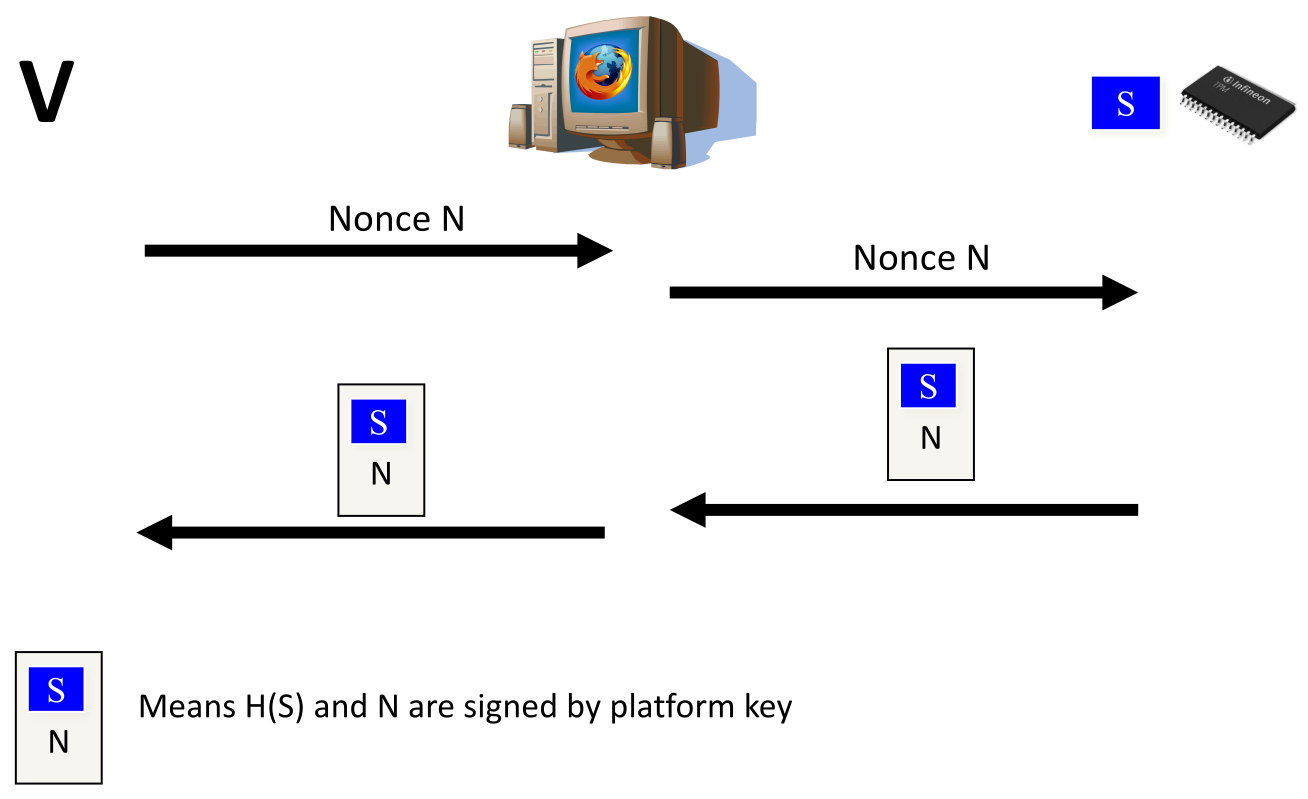
\includegraphics[width=0.8\columnwidth]{tcg-attestation.png}
      \end{center}
        \begin{enumerate}
            \item verifier sends nonce to TPM
            \item TPM returns measurements, nonce signed with platform key
        \end{enumerate}
	\textbf{Attestation says, that \textit{a} TPM signed it, but not
	\textit{which}} $\Rightarrow$ Possible attack!
    \item establish secure channel
      \begin{center}
	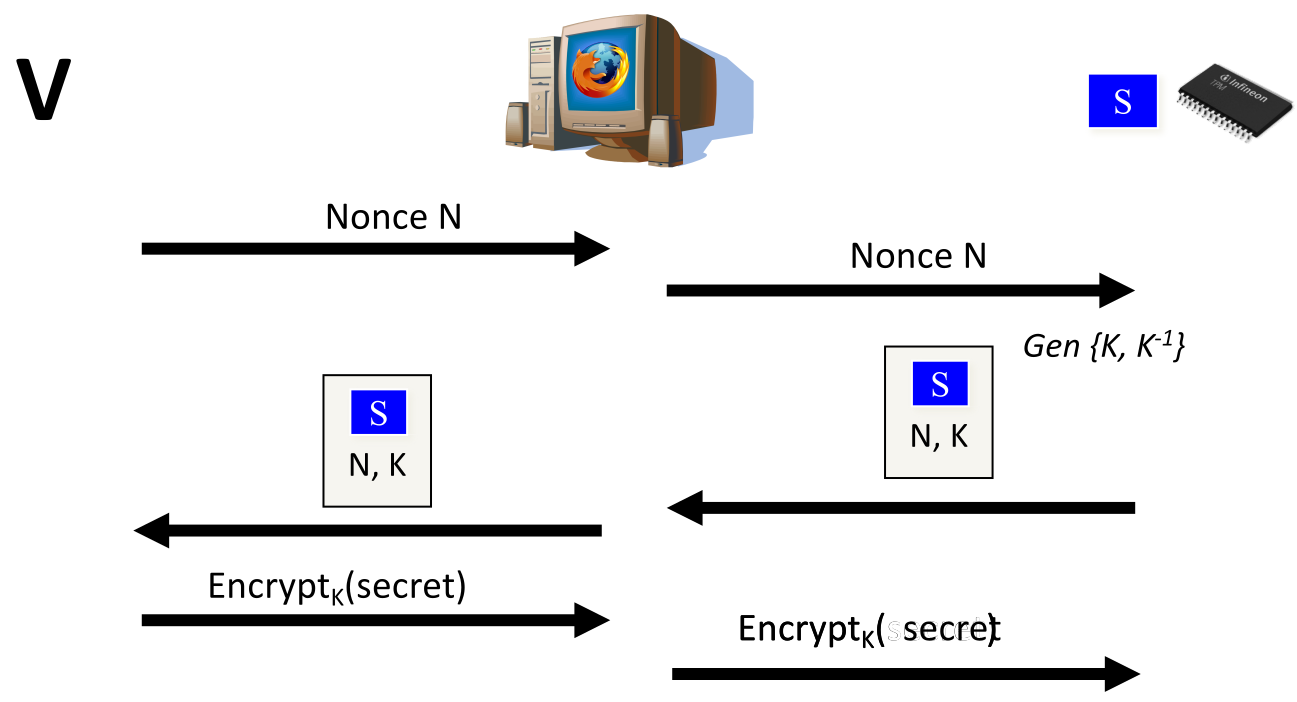
\includegraphics[width=0.8\columnwidth]{tcg-secure-channel.png}
      \end{center}
        \begin{enumerate}
            \item verifier sends nonce to TPM
            \item TPM generates $\{K, K^{-1}\}$, send back $\{\texttt{measurement, nonce}, K\}$ signed with platform key
        \end{enumerate}
    \item verify output
      \begin{center}
	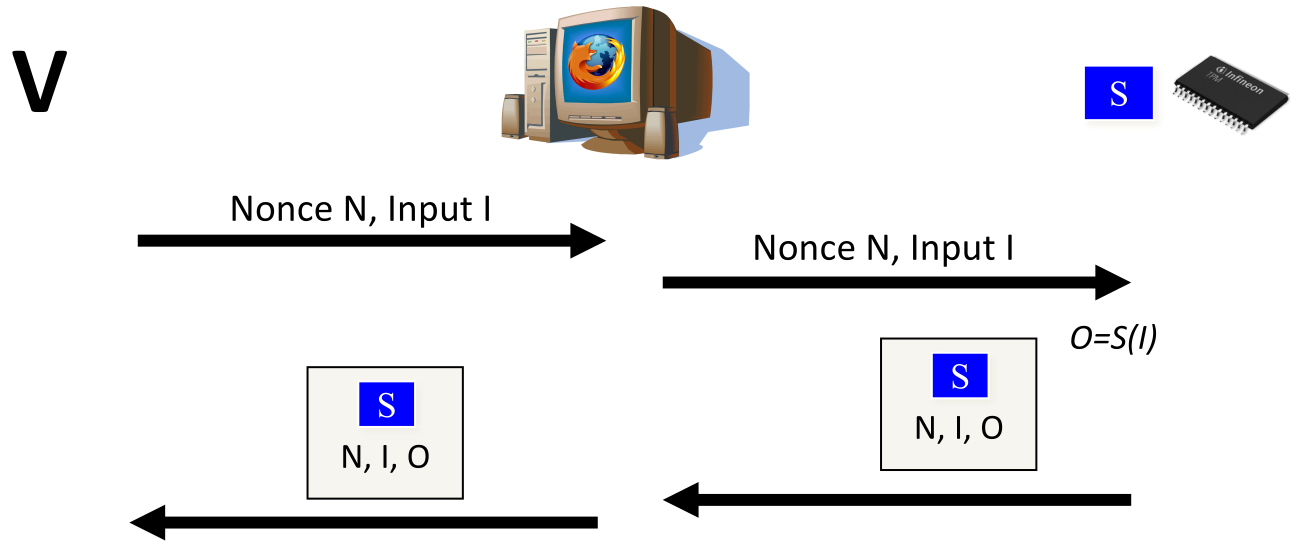
\includegraphics[width=0.8\columnwidth]{tcg-io.png}
      \end{center}
        \begin{enumerate}
            \item verifier sends nonce to TPM
            \item TPM sends back measurement, nonce, input and output signed with platform key
        \end{enumerate}
\end{itemize}

\textbf{No need to trust OS anymore, therefor minimal TCB.}

\subsection{SGX vs TPM}
SGX advantages:
\begin{itemize}
    \item Memory encryption
    \item robust against LPC-bus tampering
    \item can execute unprivileged code (ring 3)
    \item multi-threaded execution
    \item parallel execution of enclave and untrusted code
    \item enclaves can be interrupted
\end{itemize}

SGX disadvantages:
\begin{itemize}
    \item no sealed storage
    \item remote attestation requires online third party (Intel)
    \item memory access pattern reveals information about computation
\end{itemize}

	\section{Software-Only Root of Trust}
\textbf{Problem}: How can we achieve DRTM on machines without HW support such as \texttt{SKINIT/SENTER} or SGX?

\textbf{Goal}: Externally verifiable code execution without specialised HW
\subsection{Reflection}
\begin{enumerate}
    \item fill entire memory with random data
    \item clear system state and disable interrupts (secure-ish execution env)
    \item compute hash over memory
    \item return hash and system state to verifier
\end{enumerate}

Verifier checks time it took to compute response, received hash and system state.
To protect against replay attacks (or precomputed results) verifier asks for complete memory hash and two hashes over random intervalls.

\subsection{Genuinity}
Slightly different problem setting: Verifier wants to check code integrity, code execution and that the \textbf{code ran on the machine} it was expected to run on.

\begin{enumerate}
    \item verifier sends checksum code to client
    \item code uses pseudo random access pattern $\xrightarrow{}$ causes cache misses $\xrightarrow{}$ alters performance counters
    \item incorporate those hardware parameters into hash
\end{enumerate}

Simulation of the above would be significantly slower.

\subsection{SWATT}
Rellies on optimal code such that attack can not optimize to gain time.
\begin{enumerate}
    \item verifier sends nonce as seed for random access pattern
    \item walk over memory and compute hash
\end{enumerate}

Attacker would need to check and replace every memory read which reveals its presence. Time consuming task!

Infeasible for large memory. Therefor only use partial memory scans $\xrightarrow{}$ open new attack vectors such as memory copy attacks.

\subsubsection{ICE - Improved Checksum}
Include program counter and data pointer in checksum. For any memory copy attack one will differ from the original one.

\subsubsection{ICE Key Exchange}
\begin{enumerate}
    \item receive challenge from remote party
    \item compute checksum and setup TEE (disable interrupts etc.)
    \item compute secrets in TEE
    \item send back public results
\end{enumerate}

Prevents MITM attacks. Attacker can even know entire memory before protocol runs.

\subsubsection{Pioneer}
\begin{enumerate}
    \item verifiy integrity through SW attestation
    \item setup TEE
    \item setup and run code in TEE
\end{enumerate}
\begin{center}
    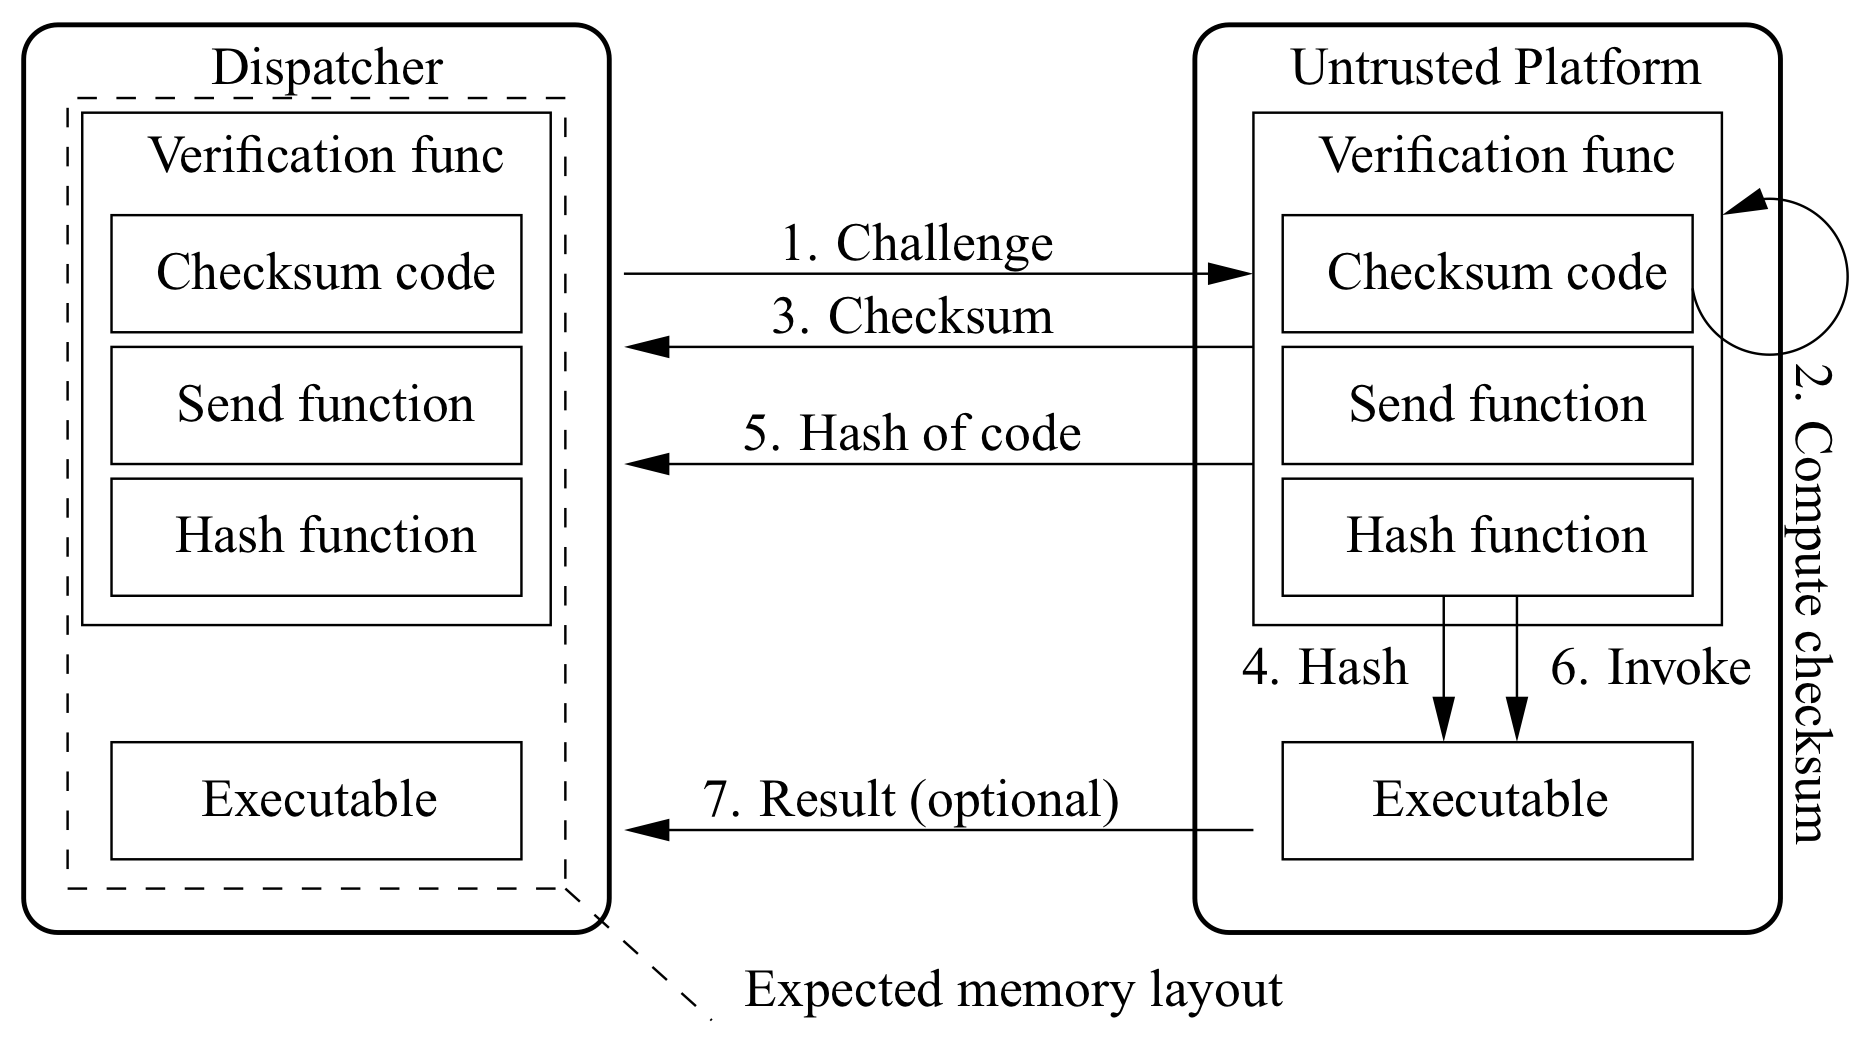
\includegraphics[width=0.8\linewidth]{images/software_attestation-pioneer.png}
\end{center}

Replace interrupt handlers to prevent attacker to interrupt verification function or executable.

\textbf{Trick}: Write checksum to stack, replace handlers right after checksum computation. If attacker causes an interrupt, the interrupt will overwrite stack with checksum $\xrightarrow{}$ attestation fails.

\textbf{Drawback:} Requires defense against proxy and overclocking attack.

	% !TeX root = ../summary-syssec.tex

\section{IoT}
\subsection{Light bulbs go nuclear}
\begin{enumerate}
    \item extract firmware update signing key using differential power analysis
    \item circumvent proximity checks
    \item make bulb join malicious network
    \item perform OTA firmware update
\end{enumerate}
Note: classical defence mechanisms like firewalls are not effective

Works because firmware only includes a MAC and is not signed (asymmetrically), therefor extracted key can \textit{sign} new firmware updates.

\subsubsection{IoT Stack}
\begin{center}
    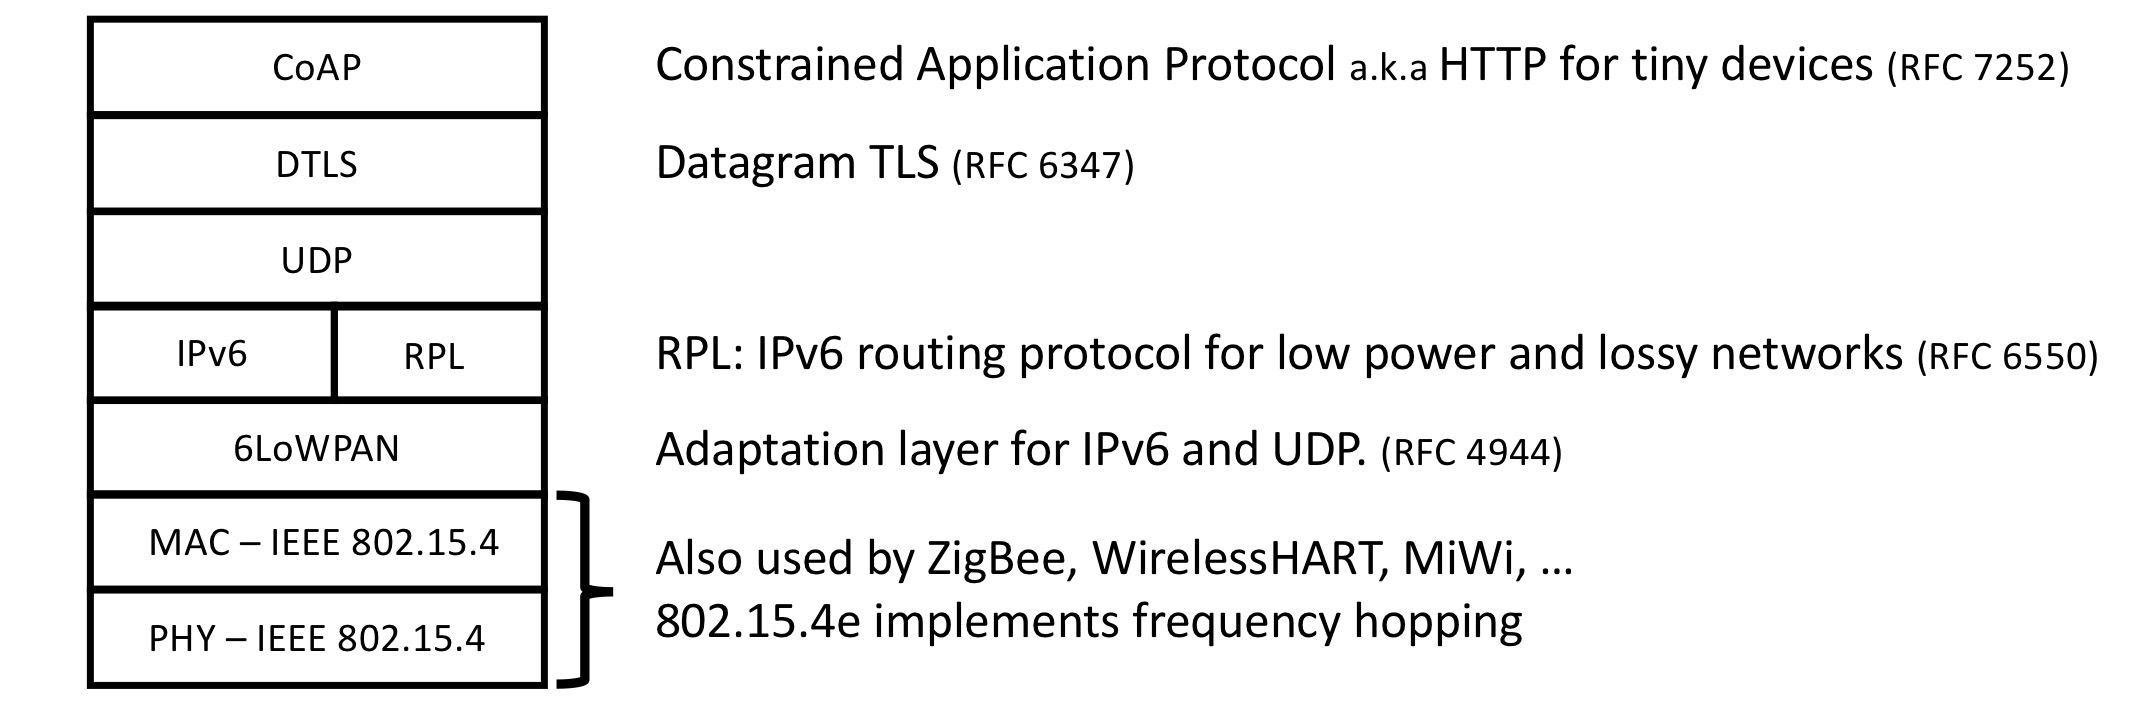
\includegraphics[width=\linewidth]{images/iot_stack}
\end{center}

\subsubsection{Encrypt everything?}
\textbf{Not sufficient}! device identifiers, traffic volume still leak information, activities

\begin{description}
  \item[existential leakage] single transmission implies real-world event
    \begin{itemize}
      \item Can not be fully eliminated
    \end{itemize}
  \item[statistical leakage] deviation from normal implies real-world event
    \begin{itemize}
      \item Can be eliminated.
    \end{itemize}
\end{description}

\subsubsection{Hide transmission times and encrypt?}
\textbf{Not sufficient}! Examples:
\begin{itemize}
    \item VOIP word reconstruction from encrypted packages (leak from variable bit length encoding and length-preserving encryption).
    \item side-channel leaks of web apps by analysing traffic
\end{itemize}

\subsection{Device Pairing}
\begin{description}
    \item[Pairing] process of establishing a security association between two devices without prior shared knowledge
    \item[security association] can be anything only known to paired devices (e.g. secret key)
\end{description}

Paring method shall minimise I/O hardware needed and avoid complex user interactions.

\begin{description}
    \item[Out-of-band] extra channel which guarantees authenticity and is
      assumed to be secure even under MITM attack \hfill\\
      Examples:
      \begin{itemize}
      	\item Visible Light
	\item Infrared
	\item Audio
	\item Haptic
	\item Sensing
      \end{itemize}
    \item[In-band] often relies on physical channel properties and use special encoding (etc.) to detect MITM attack easily.
\end{description}

\subsubsection{Bluetooth Low Energy}
Four authentication methods supported:
\begin{description}
  \item[Just Works] provides no authentication.
  \item[Passkey Entry] displays a 6-digit PIN code on one device, and the user needs to
    type the PIN on the other.
  \item[Numeric Comparison] displays 6-digit PIN codes on both devices and the
    user needs to confirm that they are identical.
  \item[Out-of-band (OOB)] is directly provided with a shared key and assumes the key
    has been securely established via an alternative OOB channel.
\end{description}
Devices can negotiate and select one based on their I/O capabilities.

	% !TeX root = ../summary-syssec.tex
\section{Stack Attacks}
\subsection{Stack Frame}
\begin{center}
  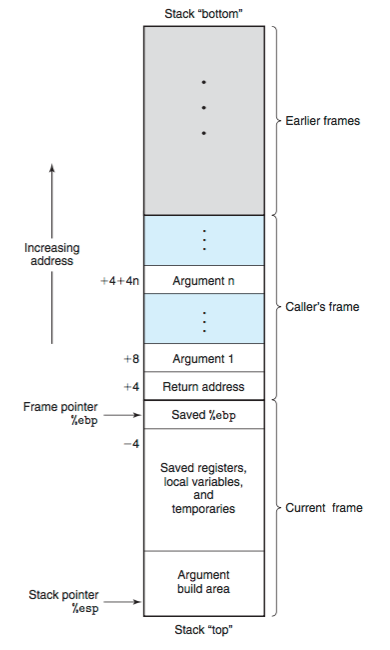
\includegraphics[width = 0.5\columnwidth]{stack-frame-structure.png}
\end{center}

\subsubsection{Construction}
The steps needed to call a function and construct a new stack frame are
\begin{enumerate}
  \item Push the last argument to the top of the stack;
  \item Push the first argument onto the stack;
  \item Push the return address onto the stack;
  \item Jumping to the called function;
  \item Saving the caller's base pointer on the stack;
  \item Move the base pointer to the top of the stack
  \item Allocating local memory for the callee.
\end{enumerate}

\subsubsection{Destruction}
The steps needed to seamlessly return and resume the execution of the parent
(caller) function are:
\begin{enumerate}
  \item Moving the stack pointer to the bottom of the callee's frame (value of
    \texttt{ebp})
  \item Restoring the caller's base pointer by popping it
  \item Taking the return address off the stack and jumping to it
  \item Freeing space allocated for the callee arguments
\end{enumerate}

\subsection{Protection}
\begin{description}
  \item[Canaries:] A known value that should never change is saved on the
    stack. If the value is checked and is not the value it should be, the
    system can conclude that there was a buffer overflow.
  \item [Address space layout randomization (ASLR):] The addresses of
    stack, heap and libraries are moved around. Because of this, the
    addresses of specific calls are different on different machines, and
    thus, an exploit won't automatically work on any machine.
\end{description}

\subsection{Format String attacks}
A program such as
\begin{lstlisting}
int main (int argc, char** argv) {
   char *name = argv[1];
   printf(name);
}
\end{lstlisting}
is vulnerable to format string attacks. Interesting inputs are:
\begin{description}
  \item[\texttt{printf(\%s)}:] This will lead the program to print out parts of
    the memory.
  \item[\texttt{printf(\%n, \&i)}:] Writes the number of characters printed so
    far to the address \texttt{\&i}.
\end{description}


\end{multicols*}

	\appendix
	% !TeX root = ../summary-syssec.tex

\section{Comparison SGX, TrustZone and TCG}
\begin{tabular}{@{}llll@{}}
\toprule
                & SGX & TrustZone & TCG  \\ \midrule
  Execution environment of different apps & isolated            & same (small
  TEE OS)          &  \\
Remote attestation & defines protocol and service over third party            &
not specified          &  no third party required\\
Memory encryption & yes 	& 	& no\\
Sealed storage 	& no 		& 	& yes\\
Development    & open            & proprietary          &  \\
Support for parallelism & Yes 	& 	& No\\
Interrupt Enclaves 	& Yes 	& 	& No \\
\bottomrule
\end{tabular}

\setcounter{secnumdepth}{2}
\end{document}

